%%%%%%%%%%%%%%%%%%%%%%%%%%%%%%%%%%%%%%%%%
% Thin Sectioned Essay
% LaTeX Template
% Version 1.0 (3/8/13)
%
% This template has been downloaded from:
% http://www.LaTeXTemplates.com
%
% Original Author:
% Nicolas Diaz (nsdiaz@uc.cl) with extensive modifications by:
% Vel (vel@latextemplates.com)
%
% License:
% CC BY-NC-SA 3.0 (http://creativecommons.org/licenses/by-nc-sa/3.0/)
%
%%%%%%%%%%%%%%%%%%%%%%%%%%%%%%%%%%%%%%%%%

%----------------------------------------------------------------------------------------
%	PACKAGES AND OTHER DOCUMENT CONFIGURATIONS
%----------------------------------------------------------------------------------------

\documentclass[a4paper, 11pt]{article} % Font size (can be 10pt, 11pt or 12pt) and paper size (remove a4paper for US letter paper)

\usepackage{amsmath}
\usepackage[protrusion=true,expansion=true]{microtype} % Better typography
\usepackage{graphicx} % Required for including pictures
\usepackage{wrapfig} % Allows in-line images

\usepackage{mathpazo} % Use the Palatino font
\usepackage[T1]{fontenc} % Required for accented characters
\linespread{1.05} % Change line spacing here, Palatino benefits from a slight increase by default

\makeatletter
\renewcommand\@biblabel[1]{\textbf{#1.}} % Change the square brackets for each bibliography item from '[1]' to '1.'
\renewcommand{\@listI}{\itemsep=0pt} % Reduce the space between items in the itemize and enumerate environments and the bibliography

\renewcommand{\contentsname}{Indice} % Rename TOC default title

\renewcommand{\maketitle}{ % Customize the title - do not edit title and author name here, see the TITLE block below
\begin{flushright} % Right align
{\LARGE\@title} % Increase the font size of the title

\vspace{50pt} % Some vertical space between the title and author name

{\large\@author} % Author name
\\\@date % Date

\vspace{40pt} % Some vertical space between the author block and abstract
\end{flushright}
}

%\setcounter{tocdepth}{5}
\usepackage{hyperref} % Enables hyperlinking (e.g., ToC)

%----------------------------------------------------------------------------------------
%	TITLE
%----------------------------------------------------------------------------------------

\title{\textbf{Soccer-SCD}\\ % Title
\vspace{10pt}Simulatore di calcio - Progetto di Sistemi Concorrenti e Distribuiti} % Subtitle

\author{\textsc{Sebastiano Catellani\\Sebastiano Gottardo\\Alessandro Sforzin} % Author
\vspace{20pt}\\{\textit{Universita' degli Studi di Padova}}} % Institution

\date{\today} % Date

%----------------------------------------------------------------------------------------

\begin{document}

\maketitle % Print the title section

\newpage

\tableofcontents % Print the Table of Contents

\newpage

%----------------------------------------------------------------------------------------
%	INTRODUZIONE
%----------------------------------------------------------------------------------------

%----------------------------------------------------------------------------------------
%	INTRODUZIONE
%----------------------------------------------------------------------------------------

\section*{Introduzione}
\addcontentsline{toc}{section}{\protect\numberline{}Introduzione}%
\label{sec:introduzione}

Paragrafo introduttivo.

\subsection*{Scopo del progetto}
\addcontentsline{toc}{subsection}{\protect\numberline{}Scopo del progetto}%
\label{sec:scopo_del_progetto}

Scopo del progetto.

\subsection*{Funzionalita' del software}
\addcontentsline{toc}{subsection}{\protect\numberline{}Funzionalita' del software}%
\label{sec:funzionalita_del_software}

Funzionalita' del software.

\subsubsection*{La partita}
\addcontentsline{toc}{subsubsection}{\protect\numberline{}La partita}%
\label{sec:partita}

La partita.

\subsubsection*{Il software}
\addcontentsline{toc}{subsubsection}{\protect\numberline{}Il software}%
\label{sec:software}

Il software.

\subsection*{Obiettivi}
\addcontentsline{toc}{subsection}{\protect\numberline{}Obiettivi}%
\label{sec:obiettivi}

Obiettivi.

%----------------------------------------------------------------------------------------
%	ENTITA' COINVOLTE
%----------------------------------------------------------------------------------------

%----------------------------------------------------------------------------------------
%	ENTITA' COINVOLTE
%----------------------------------------------------------------------------------------

\section*{Analisi}

Come accennato precedentemente il software a lo scopo di creare una simulazione di una partita di calcio. Nella fase di analisi e’ stato preso in considerazione lo svolgimento di una partita, i protagonisti che ne fanno parte ed i loro ruoli all’interno del gioco. Dove necessario vengono messe in risalto le interazioni desiderate tra utente e software.

\subsection*{La partita}
\addcontentsline{toc}{subsection}{\protect\numberline{}La partita}%
\label{sec:entita_giocatori}

La partita suddivisa in due tempi di egual tempo, durante i quali i lo svolgimento del gioco prosegue secondo le regole ufficiali del calcio. All’avvio del progetto l’utente deve essere in grado di poter determinare la formazione delle squadre, quindi i giocatori che scenderanno in campo e le loro posizioni. Una volta concluso il primo tempo, che deve avvenire secondo le tempistiche di gioco in modo automatico, l’utente determina l’inizio del secondo tempo. In ogni momento il software deve mettere a disposizione la possibilita’ di fermare il gioco per farlo riprendere in un secondo momento ma anche cancellare la partita per crearne una nuova.

\subsection*{Allenatori e squadra}
\addcontentsline{toc}{subsection}{\protect\numberline{}Allenatori e squadra}%
\label{sec:entita_giocatori}

Gli allenatori sono coloro che tengono sotto controllo le squadre ed i giocatori che sono in campo. Una decisione presa dall’allenatore si ripercuote sul gioco, andando a modificare le posizioni in campo dei giocatori, il loro atteggiamento in fase difensiva ed offensiva. Inoltre, entro le regole di gioco, puo’ effettuare delle sostituzioni che stanno effettivamente giocando e quelli in panchina. L’utente agisce sull’allenatore ogni qual volta vuole per effettuare le operazioni appena citate, quindi cambio formazione e giocatori. In questo caso si necessita di una visione generale delle statistiche di ogni giocatore per rendere piu’ facile prendere decisioni su quali sostituzioni attuare.

\subsection*{I giocatori}
\addcontentsline{toc}{subsection}{\protect\numberline{}I giocatori}%
\label{sec:entita_giocatori}

I giocatori sono i protagonisti principali all’interno dello svolgimento della partita. Essi devono essere liberi di agire sul campo di gioco ed avere quindi a disposizione una serie di azioni possibili per poter portare la propria squadra alla vittoria.\\

Prima di tutto, ad ogni giocatore sono assegnate delle caratteristiche di gioco (es. velocita’, difesa, potenza, ecc.) che ne determineranno la buona riuscita o meno delle operazioni che vuole effettuare. Alcuni esempi possono meglio spiegare questo aspetto, supponiamo che un difensore voglia rubare palla all’attaccante della squadra avversaria, saranno quindi la bravura nel tackle del primo e la capacita’ del secondo di driblare a determinare la buona riuscita o meno dell’intervento. Altro esempio, se due giocatori vogliono arrivare alla stessa posizione, dove magari si trova la palla, quello maggiormente veloce arrivera’ per primo.\\

Ogni giocatore in campo deve essere in grado di decidere autonomamente in base alla situazione di gioco ed alle direttive dell’allenatore, e le azioni possibili si possono suddividere in tre gruppi: movimento nel campo, in ogni direzione per raggiungere la posizione desiderata; interagire con la palla, quindi prenderla, spostarla quando ci si muove, passarla e tirarla in porta, ed infine operazioni che comprendono un altro giocatore, per contrastare o driblare un avversario.

\subsection*{L'arbitro}
\addcontentsline{toc}{subsection}{\protect\numberline{}L'arbitro}%
\label{sec:entita_giocatori}

L’arbitro deve essere in grado di avere il controllo della situazione di gioco e valutare le azioni effettuate dai giocatori per decidere se rispettano il regolamento o se sono passibili di sanzione. Piu’ nel dettaglio, l’arbitro controlla la partita, determinandone fine primo tempo e fine secondo tempo, ferma il gioco in caso di necessita’ e permette le sostituzioni. Controlla le singole mosse dei giocatori quando vanno ad interagire tra di loro, in modo tale da rilevare eventuali scorrettezze come per esempio un fallo. Infine monitora la posizione della palla per fermare il gioco quando la palla esce o se finisce in porta, aggiornando cosi’ il risultato della partita e riportando le squadre al centro del campo.


\section*{Entita' coinvolte}

In questo capitolo viene ripresa l’analisi fatta nella sezione precedente e rielaborata per identificare le entita’ e la loro tipologia, quindi se sono entita’ attive, reattive oppure risorsa protetta, ed il loro ruolo all’interno dello scenario in cui si svolge la partita. 

\subsection*{Entita’ attiva: i giocatori}
\addcontentsline{toc}{subsection}{\protect\numberline{}Entita’ attiva: i giocatori}%
\label{sec:entita_giocatori}

Nel modello che modello che verra’ discusso in seguito i giocatori sono identificati da delle entita’ attive, quindi dotate di un proprio flusso di controllo che interagisce con le altre entita’ in gioco secondo decisioni prese autonomamente. Nel resto della relazione viene fatto riferimento al concetto di turno, consiste in un singolo ciclo di esecuzione che viene ripetuto fino alla fine della partita. Tale turno e’ diviso in fasi, questo aspetto verra’ ripreso in seguito nei prossimi capitoli.

\subsection*{Entita’ reattiva: l'arbitro}
\addcontentsline{toc}{subsection}{\protect\numberline{}Entita’ reattiva: l'arbitro}%
\label{sec:entita_abitro}

All’interno delle dinamiche del gioco reagisce alle azioni effettuate dalle altre entita’, gestendo per le varie casistiche interrompendo o meno il gioco e permettendo in momenti opportuni ad entita’ esterne alla partita di interagire con le squadre in campo.

\subsection*{Risorsa protetta: la palla}
\addcontentsline{toc}{subsection}{\protect\numberline{}Risorsa protetta: la palla}%
\label{sec:entita_palla}

In fase di analisi la palla e’ stata menzionata come componente del gioco che subisce spostamenti scaturiti da azioni dei giocatori. Essa di conseguenza e’ una risorsa protetta che detiene la posizione in cui si trova il pallone e permette ad una sola entita’ alla volta di poterla modificare.

\subsection*{Entita’ attiva: gli allenatori}
\addcontentsline{toc}{subsection}{\protect\numberline{}Entita’ attiva: gli allenatori}%
\label{sec:entita_allenatori}

Gli allenatori non sono un entita’ attiva, dato che non prendono decisioni automamente non abbiamo bisogno che essi abbiano un proprio flusso di controllo, bensi’ devono reagire a segnali che arrivano dall’esterno. Successivamente questo aspetto sara’ piu’ chiaro quando verra’ dato una visione generale del modello che comprendera’ anche componenti di distribuzione.

\subsection*{Lo stato}
\addcontentsline{toc}{subsection}{\protect\numberline{}Lo stato}%
\label{sec:entita_stato}

In fase di analisi si e' evidenziato il fatto di come un giocatore abbia bisogno di apprendere lo stato di gioco per poter decidere la sua mossa successiva. Questo porta alla luce la necessita’ di avere un luogo unico in cui detenere lo stato di gioco, ed i giocatori lo consultano ogni qual volta ne abbiano bisogno. Tale stato consiste principalmente nelle posizioni degli altri giocatori in campo e l’andamento del gioco, per esempio se la mia squadra e’ in fase offensiva o difensiva.\\
Quello che un giocatore e’ chiamato a fare e’ quindi a grandi linee ottenere lo stato di gioco in un determinato istante, calcolare la propria prossima mossa ed andare ad aggiornare lo stato in base a quest’ultima decisione.\\

Queste considerazioni evidenziano la necessita’ di aggiungere una nuova entita’ che governi lo stato, che ne garantisca l'integrita' nel proseguire del gioco e garantisca ai giocatori di poter leggere lo stato e modificarlo secondo le mosse scelte.

%----------------------------------------------------------------------------------------
%	MODELLO
%----------------------------------------------------------------------------------------

%----------------------------------------------------------------------------------------
%	MODELLO
%----------------------------------------------------------------------------------------

%\subsection{Il modello}
%\label{sec:modello}
%
%Nella Sezione~\ref{sec:entita_coinvolte} sono state individuate ed analizzate le entità che caratterizzano il sistema. La fase successiva consiste nel definire le interazioni %che legano le suddette entità, in maniera tale da poter derivare un modello per il sistema.

\subsubsection{Interazione tra giocatori: il controllore}
\label{sec:modello_interazione_giocatori}

%Interazione tra giocatori: il controllore.
I giocatori sono i principali attori del sistema. Un giocatore si sposta dentro e fuori dal campo ed è in grado di compiere diversi tipi di azioni (Sezione~\ref{sec:analisi_giocatori}), che decide sia sulla base del proprio stato che dello stato della propria squadra e della partita. Un aspetto fondamentale vede i giocatori, così come avviene nel mondo reale, operare in maniera parallela e concorrente tra di loro; inoltre, i risultati delle loro azioni debbano riflettersi sullo stato di gioco che, come descritto in Sezione~\ref{sec:entita_coinvolte_stato}, detiene tutte le informazioni che definiscono la partita in un dato istante. Si pone però un problema: i giocatori, per poter conoscere le informazioni che permetteranno loro di decidere la prossima azione da compiere, devono accedere allo stato, che tuttavia è unico. È dunque necessario regolamentare l'accesso a tale risorsa, in maniera tale da preservarne la consistenza e la correttezza.\\

La componente che si occupa di permettere l'interazione tra diversi giocatori è il \textit{controllore}. In quanto entità centrale di controllo, i suoi molteplici compiti possono essere raggruppati come segue:

\begin{enumerate}
	\item Permettere ai giocatori di accedere allo stato, sia per leggerne le informazioni sia per poterle modificare
	\item Sequenzializzare gli accessi allo stato da parte dei giocatori, al fine di non creare inconsistenze sulle informazioni in esso contenute
	\item Ricoprire il ruolo di arbitro di gioco ``onnisciente'' (verrà dettagliato in Sezione~\ref{sec:modello_verifica_arbitro})
\end{enumerate}

Come già accennato precedentemente, un giocatore decide la sua prossima mossa sulla base dello stato corrente della partita: ad esempio, trovandosi in possesso della palla nell'area avversaria e senza nessun giocatore a marcarlo, è ragionevole che il giocatore decida di tirare per provare a realizzare un goal. Al tempo stesso, l'azione che egli compie si ripercuote sullo stato della partita, andandone a modificare una parte: di nuovo, se il giocatore segna, il punteggio della partita cambia e i giocatori ritornano in posizione di partenza per ricominciare il gioco. Questo meccanismo mette in luce una necessità tale per cui le operazioni che alterano lo stato siano quanto più possibile sequenziali ed atomiche. Sebbene questo argomento verrà trattato ampiamente nel Capitolo~\ref{sec:analisi_architetturale}, è importante capire il motivo dell'importanza di queste due caratteristiche.\\

Il requisito di atomicità si rivela particolamente critico quando si assume di operare in condizioni di prerilascio dei processi. Sotto questa condizione, un processo in esecuzione può essere ``temporaneamente fermato'' (prerilasciato) in favore di un altro processo, che entra quindi in esecuzione al suo posto; una simile condizione si verifica, ad esempio, se il processo corrente ha una priorità inferiore di quello che vuole subentrare. Per spiegare come il prerilascio minacci la consistenza dello stato della partita, si consideri una situazione dove due giocatori avversari si contendono il possesso della palla, che giace inerte in mezzo a loro. Entrambi i giocatori leggono lo stato e decidono di provare a conquistarne il possesso. Si supponga che il processo relativo al primo giocatore venga prerilasciato prima di aver potuto applicare la sua mossa sullo stato. Nel frattempo, il secondo giocatore conquista la palla e si muove verso la porta avversaria. Quando il primo giocatore torna in esecuzione si trova in uno stato nel quale la mossa precedentemente decisa risulta inconsistente, in quanto lo stato è cambiato senza che lui lo sappia. Se si permettesse al primo giocatore di applicare senza alcun controllo la sua mossa si darebbe origine ad una situazione in cui entrambi i giocatori hanno il controllo della palla.\\

 Questo esempio evidenzia come non sia possibile garantire atomicità per l'intero turno di un giocatore senza inficiare il parallelismo, rischiando di ottenere un sistema puramente sequenziale. Piu' in generale, all'inizio di ogni suo turno un giocatore deve prendere coscienza di quale sia lo stato attuale di gioco, decidere la prossima mossa sulla base di quest'ultimo e sottoporla al controllore per modificare lo stato. Questo meccanismo, abbinato al fatto che i giocatore eseguono in modo potenzialmente parallelo e che ogni richiesta viene elaborata in maniera sequenziale, farebbe pensare ad una soluzione che prevede un accesso esclusivo al controllore da parte di un giocatore per tutta la durata del suo ciclo di esecuzione. Tuttavia, un approccio di questo tipo porterebbe ad un'esecuzione strettamente sequenziale del gioco, quindi atomico, e andrebbe a minare il parallelismo potenziale tra i giocatori. Dato che una soluzione di questo tipo non risulta essere desiderabile, l'approccio adottato consiste nello scomporre la routine del turno come segue:\\

\begin{enumerate}
	\item il giocatore richiede al controllore lo stato di gioco
	\item viene effettuata una fase di computazione con la quale decide la prossima mossa
	\item richiede al controllore di applicare l'azione scelta allo stato.
\end{enumerate}

Il modello che ne consegue prevede che sia solamente il controllore ad effetuare le scritture vere e proprie, sulla base delle azioni decise e sottoposte da parte dei giocatori. Tali richieste vengono valutate in modo sequenziale, andando a modificare lo stato con una azione alla volta ed evitandone così potenziali inconsistenza. Si ha quindi che la fase di lettura e la fase di scrittura (primo e terzo punto) vengono effettuate “online”, ovvero tramite accesso esclusivo al controllore; la parte di scelta della prossima azione avviene invece “offline”, quindi senza la necessità di interagire con esso. In questo modo si guadagna un parallelismo potenziale nella seconda fase, permettendo così ai giocatori di non interferire tra di loro nella decisione della prossima mossa.\\

\subsubsection{Verifica sullo stato di gioco: l'arbitro}
\label{sec:modello_verifica_arbitro}

Affiché una partita si svolga secondo le regole e le modalità stabilite dal gioco del calcio c'è bisogno di un arbitro che regoli l'andamento del gioco. Le mansioni dell'arbitro sono molteplici:

\begin{itemize}
	\item Sancire l'inizio e la fine dei tempi di gioco (inizio primo tempo - fine primo tempo - inizio secondo tempo - fine partita)
	\item Fermare il gioco e farlo riprendere in seguito (e.g. una rimessa laterale)
	\item Segnalare eventuali irregolarità da parte dei giocatori (e.g. un fallo)
	\item Tenere il conto dei gol segnati da entrambe le squadre, così da decretare il vincitore alla fine della partita
	\item Gestire le richieste di sostituzione e di cambio di formazione da parte degli allenatori
\end{itemize}

L'arbitro deve quindi essere in grado di controllare tutte le mosse dei giocatori, così come lo stato e la posizione della palla e la durata della partita fino a quel momento. Nella realtà, il ruolo dell'arbitro è assegnato ad un essere umano, che quindi non è infallibile: si pensi ad esempio ad un fallo che viene commesso irregolarmente alle sue spalle mentre lui è impegnato ad assegnare un calcio d'angolo. In questa simulazione si assume più semplicemente che l'arbitro sia ``onnisciente'', ovvero abbia la facoltà di analizzare ogni singola mossa di ciascun giocatore e della palla, in maniera da poter segnalare immediatamente ogni irregolarità oppure fermare il gioco all'occorrenza.\\

Si ha così che il controllore, descritto nel paragrafo precedente, ricopre anche il ruolo di arbitro. Questa decisione ha delle ripercussioni non solo nello svolgersi del gioco (l'arbitro è onnisciente), ma anche nell'assegnazione delle risorse di calcolo. Infatti, se l'arbitro fosse soggetto agli stessi vincoli di esecuzione dei giocatori, andrebbe a concorrere assieme a loro per l'esecuzione sulla CPU come task a sé stante; questa situazione non si verifica invece nel caso in cui sia il controllore ad essere anche arbitro, essendo l'entità centrale che si occupa di eseguire a tutti gli effetti le mosse dei giocatori. Maggiori dettagli sull'implementazione dell'arbitro verranno esposti in Sezione~\ref{sec:implemetazione_concorrenza}.\\

L'elenco delle funzioni che l'arbitro deve espletare nasconde tuttavia un punto critico su cui è opportuno soffermarsi. I primi quattro punti sono strettamente legati alla componente concorrente della simulazione, ovvero quella che vede l'interazione dei giocatori con il controllore e, in alcuni casi, l'agente di movimento. L'ultimo punto fa invece riferimento alla componente distribuita della simulazione, ovvero quella che si occupa di ricevere e gestire i comandi impartiti dagli allenatori ed eventualmente dalla finestra principale di controllo (che, come verrà esposto successivamente, coincide con la componente che mostra il campo di gioco e lo svolgersi della partita). La differenza sostanziale tra queste due tipologie di eventi è racchiusa nel fatto che gli eventi provenienti dalla componente distribuita non sono deterministici e non seguono nessuna regola di generazione, a differenza degli eventi relativi alla parte concorrente.
La presenza di due sorgenti di eventi introduce un problema significativo, ovvero l'ordine in cui l'arbitro deve processare/consumare quegli eventi. Ad esempio, si consideri una situazione dove si ha una richiesta di sostituzione per il giocatore 1 in favore del giocatore 3 e, allo stesso tempo, sia stato commesso un fallo commesso dal giocatore 1 sul giocatore 2. L'ordine in cui vengono processati questi eventi determina lo stato successivo, che diverge a seconda che si consideri prima uno oppure prima l'altro. Bisogna tenere conto, ad ogni modo, che gli eventi che vengono generati dalla componente distribuita hanno come precondizione il gioco fermo: quindi c'è una stretta dipendenza unidirezionale tra un evento singolo della componente concorrente e gli eventi della componente distribuita. L'approccio da seguire per garantire il massimo livello di correttezza temporale è quindi il seguente: l'arbitro dovrà prima processare l'evento singolo della componente concorrente (che può causare il gioco fermo, nel caso non lo fosse già) e solo poi processare gli eventi della componente distribuita, se le condizioni sono opportune.

\subsubsection{La palla in movimento: l'entità e l'agente di movimento}
\label{sec:modello_palla_agente_movimento}

%La palla in movimento: l'entità e l'agente di movimento.

La palla è una parte fondamentale del modello della simulazione, in quanto il suo possesso viene conteso dai giocatori che devono tirarla in porta, segnando un gol per la loro squadra. 

\begin{figure}[htb!]
	\centering
	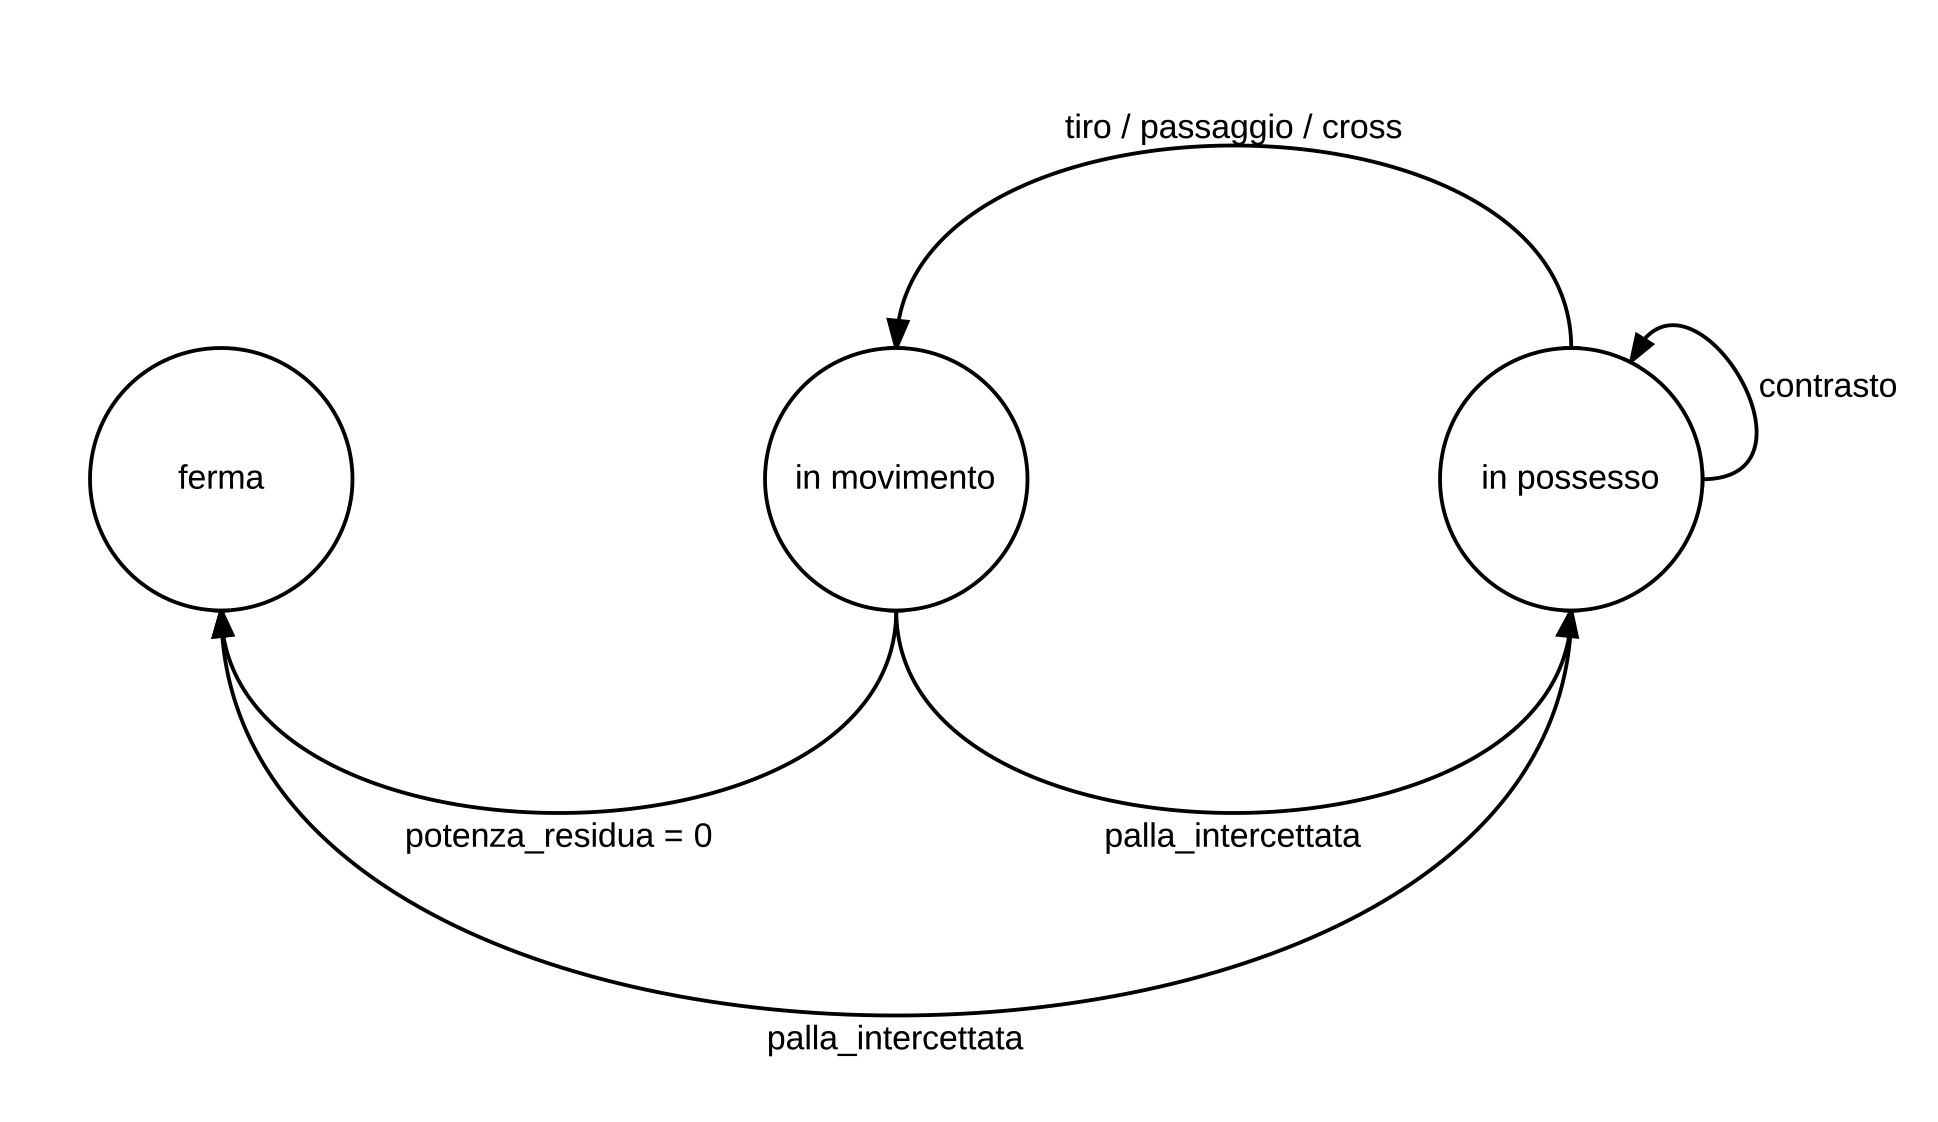
\includegraphics[scale=.8]{images/ball_state_diagram}
	\caption{Diagramma dei possibili stati della palla.}
	\label{fig:ball_state_diagram}
\end{figure}

Il suo comportamento può essere definito come una macchina a stati, schematizzato in Figura~\ref{fig:ball_state_diagram}. In ogni momento della partita, la palla occupa una delle celle del campo. Nel caso sia posseduta da un giocatore, essi condividono la stessa cella; in caso contrario, la palla occupa la cella in cui si trova. Inoltre, la palla può trovarsi solamente in due stati: quiete e moto. Una palla in movimento si può avere quando il giocatore che la controlla si sposta con essa; inoltre, si ha una palla in movimento anche quando un giocatore la passa verso un altro giocatore oppure effettua un tiro verso la porta avversaria. Al contrario, una palla è inerte se non è controllata da nessun giocatore, solitamente quando un passaggio o un tiro mancano il bersaglio (e.g. un passaggio troppo debole). La palla è quindi una risorsa protetta, che non compie azioni proprie ma che subisce azioni di altre entità attive (i giocatori) e salva di volta in volta la sua posizione aggiornata.\\

Di conseguenza, quando un giocatore effettua un passaggio oppure un tiro, la palla deve essere spostata da un'entità che però non può essere il giocatore stesso: in altre parole, si tratta di simulare l'impressione di un moto alla palla a seguito di un'azione del giocatore che la controlla. Questa mansione è ricoperta dal cosiddetto \textit{agente di movimento}. L'agente di movimento è un'entità reattiva concorrente agli altri giocatori, il cui unico compito è quello di spostare la palla in una determinata direzione fino a che la potenza ad essa impressa è sufficiente a farla avanzare alla cella successiva. Una volta completato il suo compito, smette di eseguire in attesa del prossimo spostamento da effettuare. In alcuni casi, l'agente di movimento viene volutamente bloccato attraverso l'arbitro, ad esempio nel caso in cui la palla esca dal campo e sia necessario assegnare una rimessa oppure un calcio d'angolo.

\subsubsection{Modifiche sulle squadre: gli allenatori}
\label{sec:modello_squadre_allenatori}

%Modifiche sulle squadre: gli allenatori.

Nel gioco del calcio i giocatori di ciascuna squadra vengono coordinati dal proprio allenatore, che ha il compito di scegliere come disporre i giocatori in campo (la formazione) e di effettuare delle sostituzioni, come conseguenza di un infortunio o più semplicemente per una scelta tattica. In questa simulazione i due allenatori rappresentano due componenti distribuite separate, che comunicano con l'unità centrale di controllo. Ciascun allenatore ha la facoltà di prendere le seguenti decisioni:

\begin{itemize}
	\item effettuare un cambio di formazione per la propria squadra
	\item effettuare una sostituzione di un giocatore con un suo compagno presente in panchina
\end{itemize}

Le decisioni prese da un allenatore hanno come precondizione necessaria il gioco fermo: sarà pertanto l'arbitro a dover esaminare e successivamente accettare le richieste di un allenatore solo quando le condizioni lo permettono. Nel caso di un semplice cambio di formazione, la decisione dell'allenatore viene applicata sulla squadra, cosicché i giocatori al proprio turno successivo sappiano che la loro posizione di riferimento è cambiata. Diverso e più complesso è invece il caso della sostituzione. La sequenza di operazioni che seguono una richiesta di sostituzione si possono schematizzare come segue:

\begin{enumerate}
	\item L'arbitro riceve la richiesta di sostituzione e, non appena il gioco è fermo, procede a notificarlo ai giocatori
	\item Ciascun giocatore, prima di decidere la propria mossa, controlla se l'allenatore ha deciso di sostituirlo con un compagno
	\item Nel caso del giocatore interessato alla sostituzione, esso si dirige verso la panchina (eventualmente lasciando la palla dove si trova)
	\item Una volta giunto in panchina, il suo compagno prende il suo posto in campo e si dirige verso la propria posizione di riferimento
	\item L'arbitro, ad ogni turno, controlla se il giocatore entrante ha raggiunto la posizione di riferimento e, in quel caso, sancisce la ripresa del gioco
\end{enumerate}

Il comportamento sopra descritto vale anche nel caso di più sostituzioni simultanee, che vedono i giocatori uscire ed entrare nel campo allo stesso tempo.\\

Ciascun allenatore ha inoltre una visione meno precisa del gioco e riceve pertanto un sottoinsieme degli eventi che caratterizzano una partita: dal punto di vista decisionale è infatti poco interessante per un allenatore conoscere ogni singolo movimento di ogni giocatore. Si ha quindi che l'allenatore viene notificato solo in caso di eventi ``salienti'', che come descritto nel Capitolo~\ref{sec:analisi_architetturale}, sono stati denominati \textit{Game Events}.

%\subsubsection{Gestione delle fasi di gioco: entità di gioco}
%\label{sec:modello_fasi_game_entity}
%
%%Gestione delle fasi di gioco: entità di gioco.
%
%[secondo me non va messa qui, è prettamente implementativa]


%----------------------------------------------------------------------------------------
%	ANALISI ARCHITETTURALE
%----------------------------------------------------------------------------------------

%----------------------------------------------------------------------------------------
%	ANALISI ARCHITETTURALE
%----------------------------------------------------------------------------------------

\section{Analisi architetturale}
\label{sec:analisi_architetturale}

In questo capitolo verranno presentate le decisioni architetturali inerenti la struttura e l'organizzazione del software di simulazione. L'analisi comincia con una visione generale della gerarchia di eventi, per poi suddividersi nelle scelte che riguardano la parte di concorrenza e le scelte che riguardano la parte di distribuzione.

\subsection{Gli eventi}
\label{sec:analisi_eventi}

Gli eventi sono l'elemento costituente di una partita. Essi vengono generati dalle diverse entità e possono essere raggruppati in diverse categorie. Inoltre, alcuni di questi eventi interessano la sola parte concorrente, mentre altri eventi possono viaggiare dalla parte concorrente a quella distribuita e viceversa.

\begin{figure}[htp!]
	\centering
	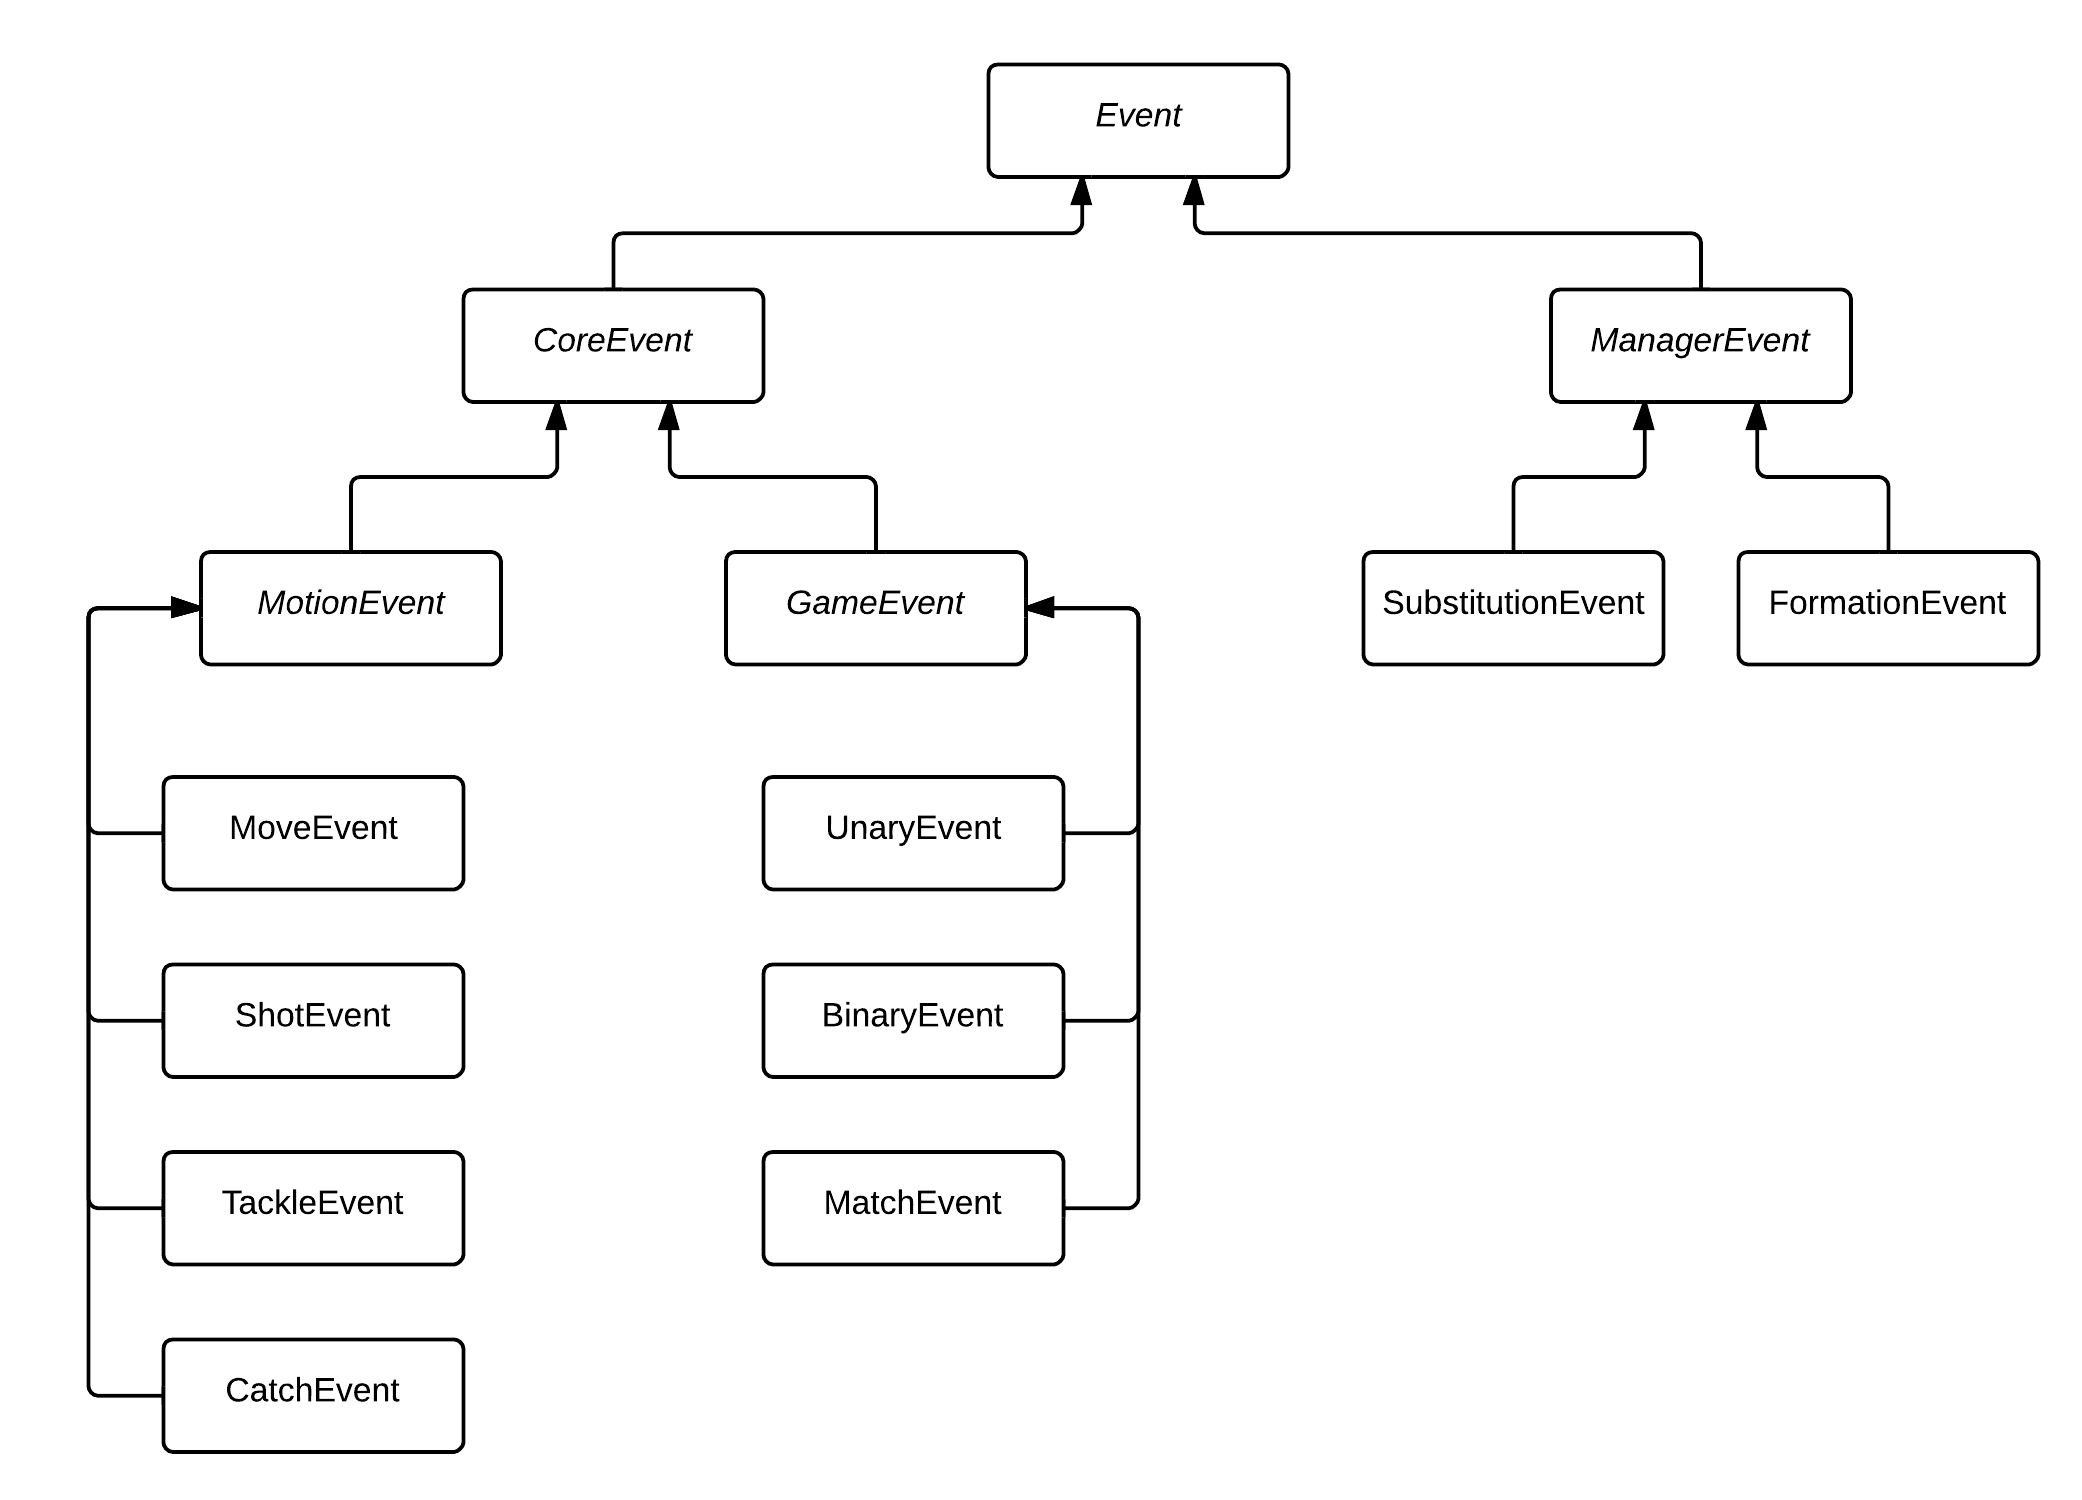
\includegraphics[scale=.2]{images/event_hierarchy.png}
	\caption{La gerarchia degli eventi che costituiscono una partita.}
	\label{fig:event_hierarchy}
\end{figure}

La struttura globale degli eventi è schematizzata in Figura~\ref{fig:event_hierarchy}. Data la sua complessità ed estensione, verranno ora trattati singolarmente i diversi tipi di eventi al fine di spiegarne il loro significato e il contesto in cui vengono utilizzati.

\paragraph{Event} \textit{Event} rappresenta l'evento generico ed è alla base della gerarchia. Da esso si diramano due macro-categorie di eventi: i \textit{CoreEvent} e i \textit{ManagerEvent}. Esso sono rispettivamente gli eventi che vengono generati nella parte concorrente (il \emph{Core}) e gli eventi che vengono generati nella parte distribuita (fondamentalmente, dagli allenatori). \textit{Event} può essere considerata come un'entità astratta, che non viene concretizzata se non da uno dei suoi derivati.

\paragraph{CoreEvent} Gli eventi di tipo \textit{CoreEvent} sono un insieme di eventi che vengono generati dalla parte concorrente del sistema. La loro generazione tuttavia non vincola il loro utilizzo nella sola parte concorrente: essi vengono infatti inviati alla parte distribuita per notificare gli allenatori (e l'interfaccia grafica del campo) aggiornamenti sullo svolgersi della partita. Vi sono due tipologie di \textit{CoreEvent}: i \textit{MotionEvent}, che rappresentano le possibili azioni dei giocatori, e i \textit{GameEvent}, che invece rappresentano tutti quegli eventi che influiscono sullo stato di gioco. Anche in questo caso, i \textit{CoreEvent} sono astratti e trovano una concretizzazione nei loro discendenti.

\paragraph{MotionEvent} Tutte le azioni che un giocatore può compiere sono definite dai \textit{MotionEvent}. Sono stati definiti quattro tipi di \textit{MotionEvent}, elencati di seguito.

\begin{itemize}
	\item \textit{MoveEvent} - descrivono i movimenti di un giocatore, dal punto in cui si trova al punto in cui si vuole spostare. Questi eventi vengono altresì usati per descrivere gli spostamenti della palla;
	\item \textit{ShotEvent} - rappresentano il tiro/passaggio effettuato da un giocatore, e sono caratterizzati da alcune informazioni quali la posizione del giocatore e la potenza impressa alla palla;
	\item \textit{TackleEvent} - corrisponde al tentativo di contrasto verso un altro giocatore;
	\item \textit{CatchEvent} - questo evento descrive il gesto di prendere possesso di una palla, sia essa inerte sul campo (non in possesso) oppure come intercettazione di una palla in movimento.
\end{itemize}

Ciascuno di questi eventi viene sottoposto all'attenzione dell'arbitro, che ne valida la correttezza nel rispetto delle regole del gioco. Inoltre, come già anticipato, questi eventi vengono anche inviati alla parte distribuita, così da poter aggiornare la visualizzazione della partita e per permettere agli allenatori di prendere decisioni tattiche.

\paragraph{GameEvent} Gli eventi che regolano lo svolgimento del gioco rientrano nella categoria di \textit{GameEvent}. Essendo una tipologia di evento molto vasta, esso si suddivide ulteriormente in tre specializzazioni: gli \textit{UnaryEvent}, i \textit{BinaryEvent} ed i \textit{MatchEvent}. Le prime due tipologie si riferiscono al fatto che l'evento coinvolge solamente un giocatore (e.g., una rimessa laterale: da qui, unario) oppure due giocatori (e.g. un fallo), mentre la terza tipologia raccoglie tutti gli eventi come l'inizio della partita, la fine del primo tempo, e così via.\\

\paragraph{UnaryEvent} Tutti gli eventi di gioco che sono raggruppati in questa categoria vanno a coinvolgere un solo giocatore per la ripresa del gioco. Essi rappresentano le seguenti situazioni:

\begin{itemize}
	\item rimessa laterale;
	\item rimessa dal fondo;
	\item calcio d'angolo;
	\item calcio di punizione;
	\item calcio di rigore.
\end{itemize}

Ciascuno di questi eventi prevede che il gioco possa essere sbloccato da un particolare giocatore della squadra interessata e che la palla sia posizionata nella posizione stabilita dall'arbitro. Il gioco può riprendere solo se i giocatori sono nella loro posizione di riferimento per quella particolare situazione, prima che la palla venga rimessa in gioco. Inoltre, questi eventi sono generati esclusivamente dall'arbitro, che per ogni azione effettuata controlla lo stato di gioco globale alla ricerca di irregolarità.

\paragraph{BinaryEvent} Questa particolare categoria vanta un solo evento possibile: il fallo. Questo evento è infatti l'unico a coinvolgere simultaneamente due giocatori di squadre opposte, e si origina quando il contrasto avviene in maniera irregolare (infortuna il giocatore, oppure compie gesti pericolosi). In questo caso l'arbitro, dopo aver segnalato del fallo, decide le modalità di ripresa del gioco, ad esempio un calcio di punizione, e genera il rispettivo evento.

\paragraph{MatchEvent} Gli eventi che regolano l'inizio e la fine di ciascun tempo di gioco fanno parte dei \textit{MatchEvent}. Di conseguenza, vi sono quattro possibili varianti: inizio del primo tempo, fine del primo tempo, inizio del secondo tempo, fine del secondo tempo. Questi eventi sono usati sia dai giocatori per capire quale azione dovranno compiere (e.g., ingresso in campo), ma vengono anche inviati alle componenti distribuite per notificare lo svolgersi della partita.

\paragraph{ManagerEvent} Questa classe astratta di eventi, al contrario dei \textit{CoreEvent} che sono generati dalla componente \textit{Core}, vengono generati dalle componenti distribuite, in particolar modo dai due \textit{Manager}. La loro funzione è quella di notificare all'arbitro una richiesta di sostituzione per un giocatore oppure di cambio di formazione. L'arbitro, una volta ricevuto l'evento, provvederà ad elaborarlo alla prima occasione utile di gioco fermo.\\

Un \textit{SubstitutionEvent} contiene informazioni quali la squadra interessata, il numero di maglia del giocatore uscente e il numero di maglia del giocatore entrante; un \textit{FormationEvent} invece, oltre alla squadra interessata, fornisce anche una sigla identificativa del nuovo assetto che la squadra dovrà assumere.

\subsection{Concorrenza}
\label{sec:analisi_concorrenza}

Questa sezione propone inizialmente una panoramica sulla soluzione scelta per garantire l'assenza di deadlock e starvation in fase di design. Successivamente viene fatta luce su casi particolari che il modello finora descritto non gestisce, mettendo in evidenza la necessità di arricchirlo con meccanismi e componenti dedicate.\\

La scelta del linguaggio per lo sviluppo della parte principale del software è ricaduta su Ada, il quale ha un modello di concorrenza che mette a disposizione una semantica molto ricca. Un aspetto molto interessante riguarda i canali di comunicazione per le richieste: questi permettono accessi potenzialmente paralleli in fase di lettura, mentre  garantiscono mutua esclusione e, in alcuni casi, anche accodamento condizionale in scrittura. Quest'ultimo costrutto è molto utile quando si vuole soddisfare una richiesta solamente al verificarsi di alcune condizioni, come per esempio una risorsa che si libera o una variazione dello stato di gioco.

\subsubsection{Deadlock, starvation e correttezza}
\label{sec:analisi_concorrenza_deadlock}

In un sistema concorrente è necessario tenere conto di problematiche come la starvation ed il deadlock, specialmente quando si è in presenza di entità che condividono risorse. Nel caso di questo progetto, i giocatori devono avere accesso ad uno stato condiviso che gli permetta di prendere decisioni, le quali andranno poi a modificare lo stato stesso.\\

L'analisi del problema ha evidenziato la necessità di avere un unico luogo in cui mantenere lo stato. In fase di modellazione, tale problematica è stata risolta ponendo un'unica entità che garantisce mutua esclusione al controllore dei dati condivisi.\\

Questa decisione rende più semplice garantire l'assenza di deadlock e di starvation. Nel secondo caso, ogni job ha la garanzia di accedere alla risorsa in un tempo finito, in quanto le richieste vengono processate con ordinamento FIFO basato sul tempo di arrivo. Per quanto riguarda invece il primo caso, è presente solamente uno dei quattro requisiti che stanno alla base di questa pericolosa condizione. I giocatori eseguono la propria sequenza di operazioni (che caratterizza un turno) dividendole tra ``online'' ed ``offline'': questo vuol dire che solamente le fasi di lettura e di scrittura necessitano dell'utilizzo della risorsa, mentre la parte di intelligenza artificiale viene effettuata in modo autonomo sui dati recuperati; inoltre, solamente la parte di scrittura richiede mutua esclusione. Il pre-rilascio non è inibito ed il suo comportamento non è controllato dal software, ma dal sistema operativo operativo sottostante: un job pre-rilasciato che sta eseguendo la sezione critica di una richiesta in mutua esclusione deterrà ancora, al suo risveglio, il privilegio sulla risorsa, mentre gli altri job che la richiedono saranno in attesa sul rispettivo canale esposto.\\

Un caso più particolare si ha invece per quanto riguarda attesa circolare ed accumulo di risorse, per cui entra in gioco un meccanismo di riaccodamento e rivalutazione delle richieste che verrà discusso in seguito. Per ora, basti sapere il concetto alla base di tale meccanismo: una richiesta che non viene soddisfatta a causa di una risorsa occupata può fallire o venire riaccodata, così da poter effettuare un nuovo tentativo di esecuzione in un secondo momento. In questo caso, dopo un certo numero di tentativi, l'operazione viene rivalutata e modificata in una simile, che vada comunque a soddisfare le esigenze del giocatore.

\subsubsection{Palla}
\label{sec:analisi_concorrenza_palla}

La palla consiste di una risorsa protetta che ne detiene la posizione e ne permette l'accesso in mutua esclusione. Si supponga di tenere tale risorsa all'interno del controllore, permettendo solo ad esso di accedervi: in questo caso, sia i giocatori che l'agente di movimento dovrebbero concorrere per andare a modificare lo stato e, di conseguenza, anche la posizione della palla: il moto della palla sarebbe quindi posto allo stesso livello delle decisioni e degli spostamenti dei giocatori. In queste circostanze verrebbe meno un fattore di realismo molto importante, tale per cui la palla è slegata dalla velocità di gioco dei giocatori in campo. Essa deve invece essere libera di muoversi a velocità molto più alte rispetto ai giocatori e deve poter continuare il proprio moto anche con gioco fermo: in quest'ultimo caso sarà l'arbitro a riposizionarla, ad esempio, in un punto opportuno a seconda dell'irregolarità. Inoltre, accodando una richiesta di movimento della palla insieme ad altre richieste dei giocatori, si rendono le operazioni strettamente sequenziali, eliminando un livello di indeterminismo desiderabile che è proprio del parallelismo e che lo avvicina al gioco reale.\\

Un chiaro esempio di questo aspetto si trova nel tentativo di un giocatore di prendere la palla in movimento. È ragionevole pensare che la sua azione possa fallire perché il tiro è troppo forte. Se invece si pongono la palla e lo stato in due luoghi differenti, diventa possibile uno scenario in cui il giocatore tenta di prendere la palla nell'ultima posizione a lui nota ma quest'ultima nel frattempo si è spostata.\\

Sulla base delle considerazioni fatte finora, all'interno dell'architettura è stato deciso di tenere le informazioni riguardanti la palla slegate rispetto al controllore. In questo modo si permette sia ad un giocatore che all'agente di movimento di contendere la palla in modo potenzialmente parallelo, demandando alla risorsa che identifica la palla gestirne gli accessi in mutua esclusione e sotto determinate circostanze.\\

La struttura della palla è stata quindi studiata in modo tale da permettere ad un entità alla volta di poterla controllare, sia essa uno dei giocatori (attraverso il controllore) oppure l'agente di movimento. Quest'ultimo si attiverà quando risvegliato da un giocatore e sarà fermato quando un altro giocatore conquista il pallone o se il moto che gli era stato impresso si è esaurito. In particolare, l'attivazione e disattivazione del task sfrutta la potenza dei canali che permettono accodamento con condizione.

\subsubsection{Giocatori}
\label{sec:analisi_concorrenza_giocatori}

I giocatori, dopo una prima fase di inizializzazione, eseguono ad ogni turno un'operazione che va a modificare sia lo stato di gioco che il proprio. Se ogni giocatore avesse la propria parte di stato, la sua condivisione con le altre entità in gioco sarebbe più complicata di quanto necessario; inoltre, la necessità di un unico stato centrale rende tali informazioni ridondanti oltre che difficilmente consistenti durante l'esecuzione della simulazione.\\

\textbf{Task stateless}\\

Utilizzando un approccio in cui i giocatori sono stateless si permette una migliore gestione dei dati condivisi, che vengono mantenuti in un unico luogo all'interno del sistema. Ad ognuno dei 22 task in campo viene assegnato un identificativo con il quale, ad ogni turno, il giocatore ottiene le informazioni che lo riguardano e di cui ha bisogno. Tale identificativo viene ottenuto in fase di inizializzazione e può cambiare solamente in caso di sostituzione tra un giocatore in campo ed uno in panchina; così facendo non vi è necessità di creare o risvegliare un secondo task.\\

\textbf{Area di azione}\\

Ogni giocatore è caratterizzato da alcune statistiche, impostate in fase di inizializzazione, che lo differenziano dagli altri: esse hanno come scopo quello di rendere lo svolgimento del gioco più realistico (Sezione~\ref{sec:analisi_giocatori}). Abbinate allo stato di gioco del giocatore stesso, rendono inoltre possibile effettuare alcune assunzioni che influiscono nello svolgimento del resto del turno.\\

Se un giocatore è in possesso della palla e tra le proprie statistiche ha un'alta precisione e potenza, esso potrà effettuare un lancio lungo e raggiungere compagni più distanti; in caso contrario, potrà sempre optare per un passaggio corto ad un compagno vicino. Viene definita in questo modo un'area di interesse del giocatore, entro la quale esso potrà agire a prescindere dall'azione che sceglierà di fare. Un giocatore che chiede al controllore lo stato di gioco della partita non necessita di avere una visione globale dell'intero campo, bensì solamente di una sua sotto parte, definita dalla sua posizione ed un raggio determinato in base alle caratteristiche del giocatore ed alle informazioni preliminari che ha ottenuto riguardo allo stato globale.\\

\textbf{Il turno}\\

La parte iniziale di ogni turno del giocatore risulta suddivisa come segue:

\begin{enumerate}
	\item richiesta al controllore del proprio stato di gioco;
	\item individuazione della posizione della palla;
	\item richiesta al controllore dello stato della propria area di interesse.
\end{enumerate}

Queste operazioni, in quanto letture, vengono effettuate potenzialmente in modo parallelo rispetto agli altri task.\\

La seconda fase consiste nella parte di intelligenza artificiale, nella quale viene decisa la prossima mossa da effettuare. Una volta decisa, viene creato il relativo evento a cui viene automaticamente abbinato un certo livello di utilità: questo valore determina quanto sia importante per il giocatore l'azione appena decisa (ad esempio, l'azione di tiro nell'area di porta avversaria assume un'importanza maggiore rispetto ad un passaggio in fase di impostazione della prossima azione). L'azione composta da evento e utilità viene sottoposta al controllore tramite una chiamata in mutua esclusione con accodamento.\\

Antecedente al ciclo di turni che caratterizzano la normale esecuzione di un giocatore è presente una fase di inizializzazione nella quale il giocatore attende che tutti i giocatori siano attivi, recupera il proprio identificativo ed attende l'inizio della partita.\\

Ci sono altri casi in cui vi è la necessità di fermare (per poi far successivamente ripartire) i giocatori: in questi casi, viene fatto uso di una risorsa protetta che mette a disposizione dei canali per accodare i giocatori, per poi sboccarli al verificarsi di determinate condizioni.\\

\textbf{Entrata in campo}\\

L'entrata in campo, così come l'uscita, è un altro degli aspetti critici della concorrenza del progetto. I giocatori sono creati con posizione di partenza sulla panchina della propria squadra, che consistono in una serie di celle esterne al campo, ed all'avvio della partita si spostano verso la propria posizione. In una partita reale i giocatori entrano ed escono dal terreno di gioco dal centro del lato lungo: al fine di ottenere questo comportamento è stata inserita una cella di campo esattamente adiacente al punto desiderato, attraverso la quale i giocatori passano dalla panchina al campo e viceversa.\\

\textbf{Sostituzione}\\

La cella utilizzata nel meccanismo di entrata ed uscita dal campo viene sfruttata anche per effettuare le sostituzioni. Un giocatore che deve essere sostituito esce fino a raggiungere tale cella e successivamente si sposta nel suo posto in panchina: lì il suo identificativo viene cambiato con quello del giocatore entrante. Dato che i giocatori non hanno stato, se non l'identificativo con il quale recuperano ad ogni turno le proprie informazioni dal controllore, modificare l'identificativo equivale ad aver effettuato una sostituzione. In questo modo vengono creati solamente 22 task in ogni partita, che vengono opportunamente riutilizzati per simulare quelli in panchina.\\

\subsubsection{Stato, controllore ed arbitro onnisciente}
\label{sec:analisi_concorrenza_controllore_arbitro}

Lo stato consiste in una serie di dati che descrivono ogni giocatore in campo: un identificativo, il numero di maglia, la posizione attuale e quella di riferimento in campo (cioè la posizione dettata dalla formazione), oltre ad informazioni generali sullo stato nel suo complesso. Lo scopo delle azioni da parte dei giocatori è quella di andare a modificare la propria posizione all'interno del campo ed effettuare altre operazioni ai fini del gioco.\\

Il controllore, avvalendosi del suo duplice ruolo di arbitro, è in grado di gestire l'andamento del gioco bloccando, quando necessario, la ricezione di azioni da parte dei giocatori.\\

\textbf{Arbitro}\\

Riprendendo quanto detto in Sezione~\ref{sec:modello_verifica_arbitro}, l'arbitro non è altro che un insieme di funzioni che il controllore svolge per garantire il rispetto delle regole del calcio.\\

In particolare, si consideri il corpo di esecuzione del controllore all'arrivo di una nuova richiesta da parte di un giocatore. In questo flusso, l'arbitro viene chiamato a seguito dell'esecuzione della mossa del giocatore ed effettua due tipologie di controlli, chiamati simbolicamente \emph{PreCheck} e \emph{PostCheck}.\\

I controlli effettuati nella fase di PreCheck sono volti principalmente a verificare, in presenza di gioco fermo, che le condizioni per la ripartenza siano soddisfatte (e.g., che tutti i giocatori siano nella loro posizione di riferimento), andando conseguentemente ad aggiornare lo stato di gioco. Inoltre, questa fase viene utilizzata anche per verificare che la sostituzione tra due o più giocatori sia stata terminata con successo.\\

La fase di PostCheck mira invece a verificare se le condizioni attuali, a seguito della mossa del giocatore, hanno i presupposti per fermare il gioco. Nell'ordine, questa fase effettua i seguenti controlli:

\begin{enumerate}
	\item verifica se l'ultima azione ha causato un fallo su un altro giocatore;
	\item controlla se ci sono eventi provenienti dalle componenti distribuite (e.g., una sostituzione) e, in caso di gioco fermo, le prende in carico;
	\item controlla se la palla è uscita dal campo e determina l'azione conseguente.
\end{enumerate}

Al termine di questa seconda fase viene impostato il nuovo stato di gioco, sulla base del quale i giocatori sceglieranno l'azione nel loro prossimo turno.

Inoltre tale canale viene sfruttato dal sistema per fermare il gioco e farlo riprendere, per esempio quando l'utente mette in pausa il gioco.\\

\textbf{Processare eventi}\\

Nel sistema esistono diversi tipi di eventi e di azioni che un giocatore può effettuare, che dal punto di vista del controllore vengono gestiti in maniera differente: una volta accettata la richiesta del giocatore, il controllore ne determina il tipo e cerca di soddisfarla, così da aggiornare lo stato con l'azione richiesta. D'altro canto, il fatto che il giocatore divida il suo turno in fasi fa sì che i presupposti secondo cui ha scelto una determinata mossa al momento della scrittura non siano ancora validi.\\

Si consideri la situazione in cui un giocatore tenta di prendere la palla che si trova in una certa posizione, ma dal momento in cui riceve le informazioni sulla posizione e quando tenta effettivamente di prenderne il possesso, la palla si è spostata. Questo comportamento, come anche in altri casi in cui ha senso applicarlo, è dettato dal desiderio di creare una simulazione realistica, in cui un giocatore non sufficientemente veloce o tardivo nell'accorgersi di una certa circostanza veda la propria azione fallire.\\

In caso di fallimento dell'operazione, ovvero a seguito di un'azione che non può più essere applicata allo stato senza creare inconsistenze, il controllore si comporta in modo differente in base al tipo di richiesta:

\begin{itemize}
	\item azioni come il passaggio, il tiro, il tentativo di prendere la palla (sia essa controllata da un avversario o meno) se non vanno a buon fine falliscono semplicemente; al turno successivo il giocatore, essendo privo di un proprio stato locale, elaborerà una nuova azione basandosi sulle informazioni fornite dal controllore;
	\item le azioni di movimento possono fallire per diverse ragioni (e.g., la cella di destinazione potrebbe essere stata occupata), ma possono essere riprovate in un secondo momento, o rivalutate se si verificano determinate condizioni
\end{itemize}

L'utilità che un giocatore assegna alla propria azione determina il comportamento del controllore nel secondo caso. Al momento dell'accettazione, la richiesta ha una certo valore di utilità (lo stesso assegnatogli dal giocatore): tuttavia, se non dovesse andare a buon fine, questo valore viene decrementato e la mossa viene messa in attesa di una nuova occasione di esecuzione. Ad ogni tentativo di esecuzione il valore di utilità decresce fino a che non diventa minore di una certa soglia fissata a priori, sotto la quale l'azione richiesta viene rivalutata dal controllore.\\

La rivalutazione viene definita come il soddisfacimento della richiesta originale attraverso un'operazione il più simile possibile a quella decisa dal giocatore. Tale meccanismo ha come scopo quello di riflettere ciò che succede nelle dinamiche di una partita reale: infatti, se un giocatore si trova improvvisamente un altro giocatore nel percorso da lui deciso, temporeggerà per un attimo (inteso come il decremento dell'utilità) nell'attesa di un suo spostamento, infine cambierà leggermente la propria traiettoria per evitare l'ostacolo.\\

Un ultimo particolare che coinvolge la rivalutazione di una mossa è il seguente. Un'azione di movimento, per poter essere di nuovo sottoposta al controllore, necessita che il giocatore che la impedisce si sia spostato. Se tale approccio fosse puntuale sulla cella del campo potrebbe risultare troppo oneroso, sia dal punto di vista implementativo che dal punto di vista dell'esecuzione. La soluzione adottata consiste nel permettere la rivalutazione delle mosse fallite di un giocatore ogni qual volta un altro giocatore lasci la propria posizione. Per rendere questo meccanismo più efficiente e scalabile è stato suddiviso il campo di gioco in 6 ``zone'' (o settori): ogni richiesta che non è andata a buon fine e deve essere ritentata viene accodata sulla zona di appartenenza della cella in cui desidera spostarsi, in attesa che un altro giocatore in quella stessa zona effettui un movimento. In questo modo non vengono rivalutate tutte le richieste accodate all'interno del controllore, ma solamente quelle che potenzialmente ora sono applicabili.\\

Riassumendo, la condivisione di risorse tra processi, se non gestita in modo appropriato, può portare a deadlock; inoltre, dal punto di vista dell'accesso allo stato, la mutua esclusione e l'approccio sequenziale garantiscono la sua assenza. Diversa invece la questione dal punto di vista delle risorse logiche: se due giocatori desiderano l'uno la cella dell'altro vi potrebbe essere una possibile situazione di stallo, in quanto entrambi detengono una risorse e non la cedono fino a che non ottengono quella desiderata. Grazie ai meccanismi descritti in questa sezione, si permette alle azioni di essere rivalutate, portando così i giocatori a modificare le proprie richieste e garantendo quindi l'assenza di deadlock anche in questo caso.

\subsubsection{La velocità}
\label{sec:analisi_concorrenza_velocita}

Nello svolgimento del gioco finora descritto le caratteristiche fisiche entrano in gioco in diversi frangenti. Quando due giocatori entrano in contatto tra di loro per contendersi la palla, ad esempio, conta soprattutto il contrasto; contano invece attacco e difesa quando un difensore tenta di rubare il pallone all'attaccante e così via. In tutti i casi è il controllore ad esaminare la richiesta di una determinata azione e a considerare le caratteristiche fisiche dei vari giocatori, decidendo quindi chi vincerà il contrasto, quanto preciso sarà il passaggio, quanto forte applicare al tiro, \ldots\\

Diverso è il discorso della velocità, per la quale è necessario un approccio differente. La velocità può essere espressa come la quantità di mosse che un giocatore è in grado di fare in un determinato lasso di tempo, che si traduce nel numero di richieste sottoponibili al controllore in questo frangente. Per semplicità di esposizione, tale quantità di tempo è identificata dal simbolo $T$, mentre con $t_0$, $t_1$, $t_2$, \ldots si indicano gli istanti a distanza $T$ durante lo svolgimento del gioco.\\

Ad ogni giocatore viene abbinato un valore tra 1 e 5 (calcolato automaticamente in base alle sue caratteristiche) per indicare quante mosse sono permesse durante $T$: di conseguenza, il giocatore con più mosse a disposizione nell'unità di tempo sarà più veloce rispetto ad un giocatore che ha un numero minore; questo numero corrisponde quindi al numero di turni che deve poter eseguire.\\

Il calcolo di $T$ è di importanza cruciale. Esso deve permettere ad ogni giocatore di eseguire un numero di volte pari al valore che rappresenta la sua velocità. Dato un campionamento del tempo di esecuzione pessimo di un turno di un giocatore, che chiameremo C, vogliamo che un giocatore lento esegua $C$ una volta all'interno di $T$, un giocatore un po' più veloce due volte, e così via fino a 5. Vogliamo inoltre che all'inizio di ogni $T$, al tempo $t_i$, tutti i giocatori siano pronti per eseguire il proprio turno: questo aggiunge al gioco un ulteriore livello di indeterminismo desiderabile, in quanto non è possibile sapere quali saranno i giocatori selezionati per eseguire per primi.\\

Da questo ragionamento si ottiene che $T$ è pari alla somma di tutti questi tempi, ovvero alla somma del tempo di tutte le esecuzioni di $C$ da parte di ogni giocatore in campo. In questo modo si garantisce ad ogni giocatore un tempo di esecuzione sufficiente per portare a termine i propri turni: spetterà poi ad ognuno di essi distribuirli in modo uniforme nell'arco di $T$, tramite un sistema di delay che scandisce il tempo.\\

\begin{figure}[htb!]
	\centering
	\exampleOne
	\caption{Esecuzione del giocatore con distribuzione dei turni.}
	\label{fig:hyperperiod_normal}
\end{figure}

Si consideri il seguente esempio. Posto $T$ pari a 40 unità di tempo, calcolato secondo gli accorgimenti appena discussi, ed iniziato al tempo $t_i$, $C$ uguale a 2 e la velocità pari a 5: il giocatore ($P_i$), tra il turno corrente e il successivo, tenterà di eseguire il suo turno entro le prime 8 (40 diviso 5) unità di tempo, per poi attendere fino a $t_i$ + 8 il prossimo turno. Tale comportamento è illustrato in Figura~\ref{fig:hyperperiod_normal}.\\

\begin{figure}[htb!]
	\centering
	\exampleTwo
	\caption{Esecuzione del giocatore con interferenza.}
	\label{fig:hyperperiod_interference}
\end{figure}

Non è detto che esso riesca ad eseguire per 2 unità di tempo nel periodo di 8, dato che i giocatori iniziano ad eseguire tutti insieme, ma di sicuro eseguirà 5 volte il tempo $C$ (2) all'interno dell'iperperiodo $T$ (40). La Figura~\ref{fig:hyperperiod_interference} porta un esempio di questo tipo, al tempo $t_i$ il giocatore non è il primo ad eseguire, attende il proprio turno e, se già passato, non aspetterà il quanto di tempo successivo.\\

Dato $C$ come stima fatta a priori, in questo meccanismo il controllore ha il compito di calcolare $T$ e tenere aggiornato il tempo $t_i$ di riferimento. All'inizio del gioco $T$ è pari alla somma di tutti i turni di ogni giocatore, ma sarà il controllore a dover poi mantenerlo aggiornato ogni qual volta ce ne sia bisogno; questo succede, ad esempio, nel caso di una sostituzione tra due giocatori, in quanto non è detto che abbiano la stessa velocità. Per quanto riguarda $t_i$, in una normale esecuzione della partita viene calcolato partendo da un tempo di riferimento all'avvio del software, al quale viene aggiunto ogni volta $T$. Nel caso di un'interruzione del gioco da parte dell'utente, invece, tale valore di riferimento viene aggiornato con l'istante in cui il gioco può riprendere.\\

\subsection{Distribuzione}
\label{sec:analisi_distribuzione}

Dal momento che la componente \textit{Core} non dispone di una propria interfaccia grafica che possa garantire la fruizione e l'interazione dall'esterno, si pone la necessità di rendere possibile una comunicazione bidirezionale da e per le componenti distribuite, ovvero \textit{Field} e le due istanze di \textit{Manager}. Di seguito verranno analizzate le soluzioni adottate per questo particolare aspetto del software, la cui rispettiva implementazione verrà trattata nel Capitolo~\ref{sec:implementazione}.

\subsubsection{Il bridge}
\label{sec:analisi_distribuzione_bridge}

Il modulo che si occupa di consentire alla componente \textit{Core} di accettare comunicazioni dall'esterno, sia in entrata che in uscita, è chiamato \textit{bridge}. A causa della duplice natura delle comunicazioni possibile, il bridge è logicamente diviso in due parti: bridge input e bridge output.

\paragraph{Bridge input}\label{sec:analisi_distribuzione_bridge_input} Il bridge input viene utilizzato dalle due componenti distribuite \textit{Field} e \textit{Manager} per comunicare con la componente \textit{Core}, occupandosi quindi di gestire tutte le comunicazioni in ingresso. Per quanto riguarda \textit{Field}, i metodi a sua disposizione permettono di:

\begin{itemize}
	\item iniziare una nuova partita;
	\item mettere in pausa la partita corrente;
	\item dare il via al secondo tempo, a seguito di un intervallo;
	\item terminare la simulazione (spegnimento globale del software).
\end{itemize}

\noindent Per quanto riguarda invece la componente \textit{Manager}, è possibile:

\begin{itemize}
	\item recuperare tutte le informazioni relative ad una squadra;
	\item recuperare tutte le informazioni relative ai giocatori;
	\item cambiare la formazione della squadra;
	\item effettuare una sostituzione tra due giocatori.
\end{itemize}

Appare tuttavia evidente che la separazione logica tra le due tipologie di bridge non rispecchia il flusso dei dati trasmessi: infatti, nel caso del bridge input, esso permette alle componenti distribuite sia di richiedere informazioni (e.g. recuperare le statistiche dei giocatori) che di inviare delle informazioni (e.g. cambiare la formazione).\\

\paragraph{Bridge output}\label{sec:analisi_distribuzione_bridge_output} Il bridge output viene invece utilizzato da \textit{Core} per notificare gli avvenimenti della partita, permettendo così a \textit{Field} e \textit{Manager} di disegnare l'interfaccia grafica e di mostrare le relative informazioni. Questo modulo gestisce quindi tutte le comunicazioni in uscita; inoltre, il flusso di dati trasmessi è solo uscente, a differenza della sua controparte.\\

Alla base del bridge output è posto un buffer, il cui compito consiste nel raccogliere tutti gli eventi di gioco che vengono generati durante una partita ed inviarli periodicamente alle componenti distribuite. Il contenuto del buffer viene inviato se si verifica una tra tre particolari condizioni. Banalmente, il fatto che il buffer si riempia completamente causa l'invio di tutti gli eventi e un conseguente svuotamento dello stesso. Se invece il buffer non riceve più eventi entro un certo periodo di tempo noto a priori, viene inviato il tutto contenuto del buffer (e viene svuotato). Infine, vi sono eventi più importanti di altri che devono essere notificati immediatamente (e.g. una fallo): anche in questo caso, il sopraggiungere di uno di questi eventi scaturisce l'invio di tutti gli eventi e lo svuotamento conseguente del buffer.\\

Ad ogni modo, la scelta della dimensione del buffer è molto importante e determina il throughtput degli eventi e la conseguente ``fluidità'' della rappresentazione grafica della partita. Tuttavia, un invio più frequente di eventi può essere causa di una congestione di rete, quindi è opportuno trovare un buon bilanciamento tra quantità di eventi inviati e frequenza di invio. A questo proposito, il bridge output applica una sorta di filtraggio degli eventi nel tentativo di unire più eventi in uno unico. Questo avviene molto spesso negli eventi di movimento dei giocatori e della palla, che sono in assoluto i più frequenti durante una partita. La tecnica che il bridge output adotta è quella di unificare delle mosse successive di uno stesso giocatore (o della palla) in un unico evento, che ha come punto di partenza quello del primo evento ricevuto e come punto di destinazione quello dell'ultimo evento ricevuto. In questo modo il numero di eventi è di gran lunga inferiore e garantisce maggior efficienza senza inficiare sulle performance e sul throughtput.\\

L'approccio appena descritto introduce però un potenziale problema per la rappresentazione grafica della partita. La mossa originata dall'unificazione di più mosse consecutive avrebbe un punto di inizio e un punto di fine molto distanti tra loro: l'effetto che si otterrebbe sarebbe una sorta di ``teletrasporto'' del giocatore, che passerebbe dalla sua posizione corrente ad una posizione molto più distante. Per prevenire questo inconveniente, ogni evento viene inviato assieme a due timestamp: il primo timestamp corrisponde alla ricezione del primo evento da parte del buffer, mentre il secondo timestamp corrisponde alla ricezione dell'ultimo evento; questo intervallo corrisponde quindi alla durata della mossa unificata. Così facendo, la rappresentazione grafica può tenere conto dell'effettiva durata di una mossa e disegnarla di conseguenza.\\

\paragraph{Utilizzo del bridge}\label{sec:analisi_distribuzione_bridge_utilizzo} Il bridge, poiché risiede all'interno di \textit{Core}, deve essere necessariamente acceduto ed utilizzato da una delle entità presenti in quella componente. Inoltre, dal momento che le comunicazioni dall'esterno sono asincrone e non predicibili, è necessario che l'accesso avvenga serialmente, sia esso in lettura o in scrittura. Per garantire questa caratteristica l'unica entità che si occupa di interagire con il bridge è l'arbitro (ai fini della spiegazione lo si consideri come un sotto-modulo del controllore). Per facilitare la comprensione delle interazioni dell'arbitro con il bridge, si consideri la seguente situazione, dove il controllore ha appena eseguito un'azione proveniente da un giocatore e la sottopone all'attenzione dell'arbitro. Quest'ultimo esegue le seguenti operazioni:

\begin{enumerate}
	\item controlla se l'azione può causare una situazione di gioco fermo (che, si ricorda, permette ad una sostituzione e ad un cambio di formazione di avvenire);
	\item interroga il bridge input e controlla se ci sono richieste da parte della distribuzione; in caso affermativo, le esegue, se le condizioni lo permettono;
	\item valida l'azione del giocatore e aggiunge il rispettivo evento alla coda del buffer di bridge output;
	\item se tale azione ne causa un'altra (e.g., un goal), l'evento di quest'ultima viene aggiunto alla coda del buffer di bridge output.
\end{enumerate}

L'ordine in cui queste operazioni vengono eseguite rispecchia l'ordine nel quale vengono processate in una vera partita di calcio. Inoltre, essendo l'accesso al bridge riservato al solo arbitro, vengono evitate potenziali inconsistenze sullo stato della partita.\\

L'unica eccezione a questa regola è costituita dagli eventi della distribuzione che agiscono sullo stato generale del sistema, ovvero la richiesta di una nuova partita, di mettere in pausa quella corrente oppure di terminare la simulazione ed il sistema. In questo caso è direttamente il bridge input ad impartire il relativo comando, senza quindi aspettare che sia l'arbitro ad accorgersi della richiesta; tale scelta è stata dettata dal fatto che questa tipologia di richieste ha la massima priorità sulle altre, in quanto agisce sul sistema stesso.

\subsubsection{Architettura client-server}
\label{sec:analisi_client_server}

La comunicazione tra le componenti distribuite \textit{Field} e \textit{Manager} e la componente centrale \textit{Core} può essere vista come una comunicazione tipica di un'architettura di tipo client-server. Generalmente, il server si mette in ascolto di eventuali richieste in ingresso: quando il client effettua una richiesta al server, questo la prende in carico, la elabora e restituisce al client la risposta. Tutto questo avviene mantenendo una connessione attiva tra le due parti, che viene terminata non appena il client riceve la risposta del server.\\

Per poter offrire le funzionalità descritte in Sezione~\ref{sec:analisi_distribuzione_bridge_input}, \textit{Core} assume il ruolo di server ed ha come client \textit{Field} e le due istanze di \textit{Manager}. All'avvio del software, \textit{Core} si mette a disposizione delle componenti distribuite, rimanendo in ascolto fino al comando di uscita. I client, una volta che \textit{Core} è avviato, possono aprire una connessione con quest'ultimo, rimanendo in attesa fino a che la loro richiesta non viene soddisfatta ed essi hanno ricevuto la rispettiva risposta.

\subsubsection{Architettura publisher-subscriber}
\label{sec:analisi_client_pusblisher_subscriber}

L'aspetto che vede \textit{Core} comunicare con le altre componenti è invece meno comune rispetto alla tipica comunicazione client-server, analizzata nella sezione precedente. Infatti, dal momento che \textit{Core} non offre nessun tipo di interazione diretta con l'utente, è necessario che le informazioni riguardanti la partita vengano inviate a \textit{Field} (per la visualizzazione e il controllo del software) e ai due \textit{Manager} (per la gestione della squadra).\\

Nonostante una soluzione possibile sia quella di replicare l'approccio precedente, che vedrebbe quindi ciascuna entità agire sia da server che da client a seconda delle necessità, non rappresenta un approccio scalabile e porterebbe un notevole aumento della complessità generale del sistema. La soluzione adottata si basa invece su un'architettura di tipo publisher-subscriber. Il suo funzionamento prevede che vi sia un fornitore di contenuti (il produttore), solitamente divisi in canali, al quale le entità interessate si iscrivono (i consumatori): ogni qual volta il produttore da origine ad un nuovo contenuto, questo viene mandato sul canale corrispondente a tutti coloro che si sono iscritti agli aggiornamenti per quel particolare contenuto. Sarà poi compito dei consumatori quello di processare correttamente il contenuto di volta in volta ricevuto.\\

Questo approccio risulta particolarmente vantaggioso in quanto mantiene una struttura chiara del sistema e non richiede alcun tipo di meccanismo di interrogazione continua (polling). Inoltre, è un approccio altamente scalabile e moderatamente trasparente per quel che riguarda il fornitore di contenuti, che ha una lista di iscritti per ciascun canale. E' tuttavia necessario che vi sia una connessione persistente tra produttore e consumatori, pena l'impossibilità del produttore di contattare direttamente i consumatori all'originarsi di un nuovo contenuto di loro interesse.


%----------------------------------------------------------------------------------------
%	AI DEI GIOCATORI
%----------------------------------------------------------------------------------------

%----------------------------------------------------------------------------------------
%	INTELLIGENZA ARTIFICIALE DEI GIOCATORI
%----------------------------------------------------------------------------------------

\section{IA dei giocatori}
\label{sec:ai_giocatori}

In questa sezione viene descritta la struttura dell'intelligenza artificiale dei giocatori.

% Programmazione Logica: Prolog
\subsection{Programmazione logica: Prolog}
Per creare il sistema decisionale dei giocatori è stato utilizzato Prolog, un linguaggio di programmazione che trova le sue radici nella logica del primo ordine.
\footnote{Durante lo sviluppo del progetto \`{e} stato utilizzato SWI-Prolog, un'implementazione open source di Prolog compatibile con ogni piattaforma e che mette a disposizione un ampio set di tools per lo sviluppo. Sito ufficiale: \href{http://www.swi-prolog.org/}{http://www.swi-prolog.org}.}.
Come tale, un programma scritto in Prolog \`{e} un insieme di predicati formati da una concatenazione di \emph{precondizioni}, ovvero dei fatti che devono essere tutti veri affinch\`{e} la \emph{testa} della clausola sia vera.

Prolog risolve le clausole utilizzando l'inferenza logica in maniera molto efficiente, ma senza nessun controllo su cicli o cammini infiniti. Ci\`{o} lo rende molto veloce se gli viene fornito un corretto insieme di clausole, ma incompleto altrimenti. Infatti la politica adottata da Prolog \`{e} quella di ``scaricare'' sul programmatore la responsabilit\`{a} di scrivere programmi corretti ed efficienti.\\

\subsection{Struttura dell'IA}
\label{sec:struct_ia}
In questa sezione viene analizzata la struttura dell'intelligenza artificale creata in Prolog.

Il sistema \`{e} diviso in due parti principali ciascuna delle quali \`{e} composta da una serie di predicati logici scritti in Prolog. La prima parte \`{e} formata da predicati che descrivono quello che il giocatore sa riguardo a ci\`{o} che lo circonda, detta anche \emph{base di conoscenza}. Per costruirsi tali predicati ciascun giocatore deve procurarsi informazioni riguardanti la situazione in prossimit\`{a} della sua posizione (la sua posizione, quale squadra ha la palla, quali giocatori sono vicini a lui e cos\`{i} via) interrogando lo stato.

Pi\`{u} precisamente, per ciascuna informazione che il giocatore chiede ed ottiene dallo stato, viene costruito il corrispondente predicato logico scritto in Prolog. Vi sar\`{a} quindi, ad esempio, un predicato per la posizione del giocatore, un predicato per la posizione della palla, un predicato per ciascun giocatore presente nelle vicinanze del giocatore corrente e cos\`{i} via. Ovviamente nello stato sono presenti tipi di dato non interpretabili da Prolog. \`{E} quindi necessario un passaggio intermedio che ci permetta di trasformare le informazioni contenute nello stato in un formato comprensibile a Prolog. \\
Questa conversione \`{e} molto semplice ed avviene man mano che il giocatore riceve dati dallo stato. Prendiamo come esempio la posizione attuale del giocatore. Il giocatore richiede allo stato questa informazione, il quale gli restituisce un oggetto di tipo \emph{Coordinate}, un tipo di dato che rappresenta la posizione con una coppia di interi (x,y). A questo punto avviene la conversione. Dall'oggetto di tipo Coordinate sono estratti i due interi x e y, i quali vengono inseriti in una nuova stringa contenente la posizione del giocatore, scritta sotto forma di predicato logico capibile da Prolog. Se supponiamo che la posizione del giocatore presente nello stato sia la coppia di interi (10,15), la corrispondente stringa generata sarebbe: 

\begin{equation*}
	\texttt{ position(10, 15).} 
\end{equation*}

Questa operazione viene ripetuta per tutte le richieste che il giocatore fa allo stato al fine di ottenere un quadro generale di ci\`{o} che sta succedendo nella partita.\\
Una volta esaurite tutte le richieste allo stato, le varie stringhe cos\`{i} ottenute vengono concatenate in un'unica nuova stringa, che rappresenterà la base di conoscenza del giocatore. Questa nuova stringa viene passata come parametro, tramite uno script adibito all'esecuzione del motore di Prolog e alla ricezione del risultato dell'inferenza logica effettuata sulla base di conoscenza fornita come parametro, alla seconda parte del sistema.

Questa seconda parte \`{e} formata da predicati che rappresentano le azioni che i giocatori possono effettuare. A sua volta, essa si suddivide in tre categorie principali:

\begin{itemize}
	\item \emph{Actions}: contiene tutte le clausole riguardanti le azioni che un giocatore `normale' pu\`{o} effettuare. Le categorie di azioni a disposizione di un giocatore sono passaggio (\emph{pass}), tiro (\emph{shot}), movimento (\emph{move}), contrasto (\emph{tackle}) e `prendi la palla' (\emph{catch}); 
	\item \emph{Keeper}: comprende le azioni che il giocatore pu\`{o} fare se assume il ruolo di portiere. Il motivo dell'introduzione di questa distinzione tra giocatore `normale' e portiere \`{e}  che il primo non solo ha a disposizione pi\`{u}  azioni possibili rispetto al secondo, ma ha anche un comportamento differente. Ci\`{o}  non dovrebbe sorprendere visto che durante la partita il portiere sta la maggior parte del tempo fermo nella sua porta, mentre un giocatore normale si sposta nel campo ed interagisce con altri giocatori molto pi\`{u}  spesso. Inoltre alcuni eventi di gioco non interessano minimamente il portiere, come ad esempio una rimessa laterale o un semplice calcio di punizione eseguito vicino alla met\`{a}  campo, mentre il giocatore normale potrebbe dover spostarsi in una posizione particolare a causa di essi. Le azioni contenute in questo file sono quindi in numero minore e, in alcuni casi, eseguite diversamente. Per tutti questi motivi \`{e}  stato ritenuto opportuno utilizzare un set di azioni `personalizzato' solo per il portiere, nel qual caso durante l'esecuzione del programma i predicati in `Keeper' verranno utilizzati al posto dei predicati in `Actions';
	\item \emph{Utilities}: contiene clausole ausiliarie utilizzate dai predicati in `Actions' e `Keeper'. Alcuni esempi di clausole ausiliarie sono l'aggiunta di un elemento ad una lista, il calcolo della distanza tra due punti e il calcolo della corretta coppia di coordinate in cui spostarsi. Queste clausole sono state inserite in un modulo distinto per facilitare la comprensione del programma finale.
\end{itemize}

Le azioni che possono essere scelte dal giocatore in un dato momento sono determinate dallo stato della partita, dalla presenza di eventi specifici (rimessa, punizione e così via) e dalla situazione specifica nelle vicinanze del giocatore. Pi\`{u} precisamente, l'azione da compiere in un dato istante \`{e} il risultato di un'inferenza logica effettuata sulle clausole incluse nella base di conoscenza del giocatore, ovvero sull'input ricevuto dalla prima parte del sistema.

\subsection{Workflow}
Il processo decisionale che porta il giocatore ad eseguire un'azione \`{e} quindi il seguente:
\begin{enumerate}
 \item Il giocatore interroga lo stato per ottenere informazioni riguardanti le sue immediate vicinanze e lo stato complessivo della partita
 \item L'algoritmo di conversione delle informazioni da tipo di dato Ada a stringhe contenenti i predicati scritti secondo i formalismi di Prolog elabora i dati ottenuti dallo stato
 \item Viene lanciato, tramite un apposito script, il motore Prolog fornendo come input la concatenazione di predicati ottenuta al passo precedente
 \item Prolog esegue un inferenza logica sull'input ricevuto al passo precedente e fornisce in ouput la mossa ottimale per il giocatore data la situazione corrente
 \end{enumerate} 
\noindent La mossa ottenuta in output \`{e} ricevuta sotto forma di stringa Ada contenente un predicato Prolog costituito dalla mossa da effettuare e una coppia di interi (x,y) che rappresentano la coordinata sulla quale il giocatore andr\`{a} ad effettuare la mossa. Questa stringa viene scomposta in tre sottostringhe: una contenente la mossa da effettuare (ad esempio \emph{shot}, il che sta ad indicare che il giocatore ``ha deciso'' di tirare), una stringa per la componente x della coordinata e infine una per la componente y. A partire da queste sottostringhe viene creata la mossa che il giocatore cercher\`{a} di scrivere sullo stato, avendo cura di creare un oggetto di tipo \emph{Coordinate} a partire dalle due sottostringhe contenenti le componenti della coordinata finale.

\subsection{Problematiche}
\label{sec:ai_problematiche}

Verso la fase finale del progetto ci si è resi conto di un problema prestazionale che vedeva i giocatori impiegare un tempo esageratamente alto per completare il proprio turno. Dopo un'analisi inziale, il collo di bottiglia è stato identificato con la parte che riguarda la scelta della prossima mossa, quindi il processo decisionale che riguarda Prolog.\\

Inizialmente, l'approccio naîve adottato consisteva nell'invocare il motore di Prolog attraverso una libreria Java, dove sia input che output passavano attraverso dei file temporanei. Questo comportava un overhead dovuto all'istanziazione di una JVM (Java Virtual Machine) per giocatore, unita all'input/output su disco. Successivamente, si è optato per la generazione di eseguibili a partire dalle clausole di Prolog, opportunamente generate in Ada. Questo approccio ha notevolmente ridotto il tempo di esecuzione di ciascun turno, ma tale tempo continuava ad essere alto. Il problema sembra quindi essere dovuto all'elevato numero di istanze del motore di inferenze di Prolog (una per giocatore), che in alcuni casi porta ad un aumento sensibile del tempo di calcolo.\\

È stato valutato il passaggio ad un motore inferenziale di Prolog interamente scritto in Ada, tuttavia la sua implementazione era basata su un motore inferenziale unico, rendendo così impossibile un'invocazione parallela da parte di più giocatori. Si è quindi deciso di mantenere la soluzione corrente e arginare, per quanto possibile, il problema.

%----------------------------------------------------------------------------------------
%	IMPLEMENTAZIONE
%----------------------------------------------------------------------------------------

%----------------------------------------------------------------------------------------
%	IMPLEMENTAZIONE
%----------------------------------------------------------------------------------------

\section{Implementazione}
\label{sec:implementazione}

Paragrafo introduttivo.

\subsection{Concorrenza}
\label{sec:implemetazione_concorrenza}

Concorrenza.

\subsection{Distribuzione}
\label{sec:implementazione_distribuzione}

La comunicazione tra la componente \emph{Core} e le componenti \emph{Field} e \emph{Manager} è stata realizzando aggiungendo un modulo a \emph{Core} che agisce come web server. Per rendere possibile questa interazione si è ricorsi all'utilizzo di AWS (Ada Web Server). All'avvio del sistema, viene inizializzato un web server su \emph{localhost:28000}, a cui \emph{Field} e \emph{Manager} si connettono e con il quale successivamente scambiano informazioni.\\

Come già illustrato in Sezione~\ref{sec:analisi_client_server}, la comunicazione tra le componenti distribuite \emph{Field} e \emph{Manager} e la componente centrale \emph{Core} \`{e} stata implementata con un modello di comunicazione tipico di un’architettura client-server. Si ha quindi che ciascuna istanza di \emph{Manager}, una volta avviata, invia una richiesta HTTP di tipo GET a \emph{Core}, richiedendo le statistiche dei giocatori della squadra. La componente \emph{Field} effettua invece chiamate HTTP di tipo GET verso \emph{Core} al fine di richiedere azioni quali l'avvio di una nuova partita, l'avvio del secondo tempo della partita corrente, la messa in pausa della partita corrente, ed infine la terminazione forzata della partita.\\

Dal momento che \textit{Manager} e \textit{Field} sono state realizzate in Java, per facilitare tale tipo di comunicazione \`{e} stata utilizzata la libreria open source Apache HttpComponents, che fornisce una completa implementazione del protocollo HTTP in Java e consente di avere accesso a funzionalit\`{a} avanzate e maggiore flessibilit\`{a} rispetto al package standard \emph{java.net} di Java.\\

[SI E' CAPITO CHE USIAMO JAVA?]\\

In generale, le richieste provenienti da \emph{Field} e \emph{Manager} sono inizialmente ricevute dal modulo \emph{Soccer.Server.Callbacks} che si occupa di verificare di quale tipo di richiesta si tratta (i metodi a disposizione delle componenti distribuite sono consultabili in sezione ~\ref{sec:analisi_distribuzione_bridge_input}), per poi inoltrarla correttamente verso la componente \emph{Core} tramite il modulo bridge input. Nel caso in cui il client richiedente attenda una risposta da \emph{Core} (e.g. il client ha chiesto le statistiche dei giocatori), il modulo \emph{Soccer.Server.Callbacks} si occuper\`{a} di fornirla al client.\\

La comunicazione di \emph{Core} con le componenti distribuite \emph{Field} e \emph{Manager} \`{e} invece vista come un modello di comunicazione di tipo publisher-subscriber. \emph{Core} mette infatti a disposizione i seguenti canali di comunicazione ai quali le componenti interessate si iscrivono per ricevere informazioni:

\begin{itemize}
	\item \emph{/managerVisitors/registerForStatistics} \`{e} il socket su cui una delle istanze di \emph{Manager} rimane in ascolto, in particolare l'istanza che rappresenta la squadra che gioca ``fuori casa'';
	\item \emph{/managerHome/registerForStatistics} \`{e} il socket su cui una delle istanze di \emph{Manager} rimane in ascolto, in particolare l'istanza che rappresenta la squadra che gioca ``in casa'';
	\item \emph{/field/registerForEvents} \`{e} il socket a cui si connette \emph{Field}.
\end{itemize}

Per realizzare questo tipo di comunicazione si è deciso di utilizzare la tecnologia dei WebSocket. Questo particolare tipo di socket mantiene attivo un canale di comunicazione tra due componenti, ad esempio \emph{Core} e \emph{Field}, permettendo cos\`{i} la fruizione di contenuti di \emph{Core} da parte di \emph{Field}. Il principale vantaggio nell'utilizzo dei WebSocket consiste nel fatto che l'invio di nuovi contenuti disponibili da parte dell'entit\`{a} produttore verso le entit\`{a} consumatori [O CONSUMATORE?] avviene senza alcuna richiesta o sollecitazione da parte dei consumatori: non appena \`{e} disponibile un nuovo contenuto, il produttore lo invia autonomamente ai consumatori, i quali sono in ascolto sui corrispondenti WebSocket aperti. Le istanze di \emph{Manager} riceveranno informazioni riguardanti le statistiche dei giocatori e la formazione della squadra, mentre \emph{Field} riceve tutti gli eventi correlati con la partita in corso.\\

[C'E' QUALCHE CONSUMATORE DI TROPPO]

In fase decisionale si è osservato che l'accoppiamento tra la componente \emph{Core} e il server per la comunicazione con le altre componenti potesse non essere desiderabile. Ad ogni modo, si è deciso di procedere ugualmente con questa decisione, sacrificando una parte di disaccoppiamento del sistema in favore dell'uso di una tecnologia relativamente nuova ed interessante come quella dei WebSocket, che è risultata essere estremamente affidabile e di facile utilizzo.\\

Ada Web Server mette a disposizione una serie di API per facilitare l'uso dei WebSocket. Per aprire un nuovo socket \`{e} sufficiente utilizzare la funzione \emph{Register}, passando come parametro l'indirizzo su cui renderlo disponibile. Per inviare informazioni viene messa a disposizione la funzione \emph{Send}, specificando il WebSocket sul quale spedire i dati assieme alla tipologia di dato che si sta trasmettendo.\\

Come spiegato in sezione ~\ref{sec:analisi_distribuzione_bridge_output}, non vi \`{e} un continuo flusso di informazioni verso le componenti distribuite, ma viene utilizzato un buffer all'interno di bridge output, il cui scopo \`{e} bilanciare l'invio di dati: se da un lato un throughtput troppo basso comprometterebbe la rappresentazione grafica della partita, dall'altro un invio troppo frequente di aggiornamenti potrebbe causare una congestione di rete.

\subsubsection{Codifica delle Informazioni}
Tutti i messaggi scambiati secondo i modelli appena descritti sono codificati utilizzando il formato JSON, un formato di testo completamente indipendente dal linguaggio di programmazione, ma utilizza convenzioni conosciute dai programmatori di linguaggi della famiglia del C (come C/C++/C\#, Java/JavaScript e molti altri). Questa caratteristica fa di JSON un linguaggio ideale per lo scambio di dati.\\

La componente \emph{Core} processa i dati ricevuti in formato JSON utilizzando \emph{GNATColl}, o GNAT Component Collection, una libreria che mette a disposizione degli ADA package general purpose aggiuntivi. Tra di essi vi \`{e} il package \emph{GNATColl.JSON}, il quale permette sia la creazione di oggetti JSON che il parsing di tale tipo di dati ricevuti da \emph{Core}.\\

Per gestire le informazioni in formato JSON, le componenti distribuite, \emph{Manager} e \emph{Field}, utilizzano \emph{Gson}, una libreria open source  inizialmente sviluppata da Google. Questa libreria \`{e} stata scelta per la semplicit\`{a} d'uso e la versatilit\`{a} delle API messe a disposizione. La conversione di un oggetto Java nella sua rappresentazione in JSON \`{e} effettuata utilizzando il methodo \emph{toJson()} messo a disposizione dalla libreria. Similmente, la conversiona di una semplice stringa JSON nel corrispondente oggetto Java \`{e} possibile utilizzando il metodo \emph{fromJson()}.

\subsubsection{Interfacce Grafiche}
Le GUI delle componenti \emph{Field} e \emph{Manager} sono state realizzate utilizzando il linguaggio Java. Questa scelta \`{e} stata guidata dal fatto che Java \`{e} un linguaggio che garantisce un certo livello di portabilit\`{a} del sistema. In particolare, la grafica ed il layout sono stati implementati utilizzando il framework Swing di Java.

[JAVA? HAI DETTO JAVA PER CASO?]

%----------------------------------------------------------------------------------------
%	COMPILAZIONE ED ESECUZIONE
%----------------------------------------------------------------------------------------

%----------------------------------------------------------------------------------------
%	COMPILAZIONE ED ESECUZIONE
%----------------------------------------------------------------------------------------

\section{Compilazione ed esecuzione}
\label{sec:compilazione_esecuzione}

Per la compilazione e l'esecuzione del progetto sono necessari i seguenti software:\\

\begin{itemize}
	\item GNAT\_GPL, ambiente di sviluppo;
	\item AWS, web server scritto in ADA;
	\item XMLAda, librerie per il parsing XML;
	\item GNATColl, una libreria che mette a disposizione degli ADA package aggiuntivi; 
	\item Java utilizzato nello sviluppo delle interfacce grafiche;
	\item Prolog, in particolare SWI-Prolog, utilizzato nello sviluppo dell'intelligenza artificiale dei giocatori;
	\item Ada Util, un insieme di packages per Ada che forniscono funzionalit\`{a} aggiuntive.
\end{itemize}

\noindent Tutti questi software sono gratuiti e liberamente scaricabili. In particolare GNAT\_GPL, AWS, XMLAda e GNATColl sono sviluppati e supportati da Ada-Core e sono disponibili al sito http://libre.adacore.com sotto licenza GPL. Bisogna inoltre fare attenzione ad avere una versione di Java non inferiore a Java 6. Come detto in precedenza l'implementazione di Prolog utilizzata \`{e} SWI\_prolog, scaricabile gratuitamente dal sito http://www.swi-prolog.org/ in licenza LGPL. Infine Ada Util \`{e} reperibile al sito http://code.google.com/p/ada-util/ in licenza Apache 2.0. 

Il progetto \`{e} stato testato nelle distribuzioni Linux Ubuntu e Mint e in Mac OS X.

\noindent Di seguito vengono proposti i passaggi da eseguire per avere un ambiente di sviluppo pronto, in grado di compilare il progetto. La distribuzione di riferimento \`{e} Mint desktop 15 i386. Per ulteriori dettagli si pu\`{o} far riferimento ai file README o INSTALL presenti negli archivi dei file scaricati.
\begin{itemize}
	\item Scompattare [GNAT FILE]
		\begin{itemize}
			\item[] installare l'ambiente con il comando ./doinstall
			\item[] esportare le variabili d'ambiente in questo modo
			\item[] export PATH=/usr/gnat/bin:\$PATH
			\item[] export GPR\_PROJECT\_PATH=/usr/gnat/lib/gnat
			\item[] export ADA\_PROJECT\_PATH=/usr/gnat/lib/gnat
		\end{itemize}
	\item Scompattare [XML ADA FILE] e lanciare i comandi
		\begin{itemize}
			\item[] ./configure --prefix=/usr/gnat
			\item[] make all
			\item[] make install (eseguire da root)
		\end{itemize}
	\item Scompattare [AWS FILE] e lanciare i seguenti comandi
		\begin{itemize}
			\item[] make setup
			\item[] make build
			\item[] make install (eseguire da root)
		\end{itemize}
	\item Scompattare [GNATCOLL FILE] e lanciare i seguenti comandi
		\begin{itemize}
			\item[] ./configure
			\item[] make
			\item[] make prefix=/usr/gnat install (eseguire da root)
		\end{itemize}
	\item [AUNIT]
	\item [ADA UTIL]
	\item L'installazione di SWI-Prolog \`{e} abbastanza semplice, in quanto gli sviluppatori mettono a disposizione un repository comodamente aggiungibile al package manager di Ubuntu e di tutte le distribuzione basate su Ubuntu 
		\begin{itemize}
			\item[] sudo apt-add-repository ppa:swi-prolog/stable
			\item[] sudo apt-get update
			\item[] sudo apt-get install swi-prolog
		\end{itemize}
\end{itemize}

\noindent A questo punto l'ambiente di sviluppo \`{e} pronto. Per compilare ed eseguire il progetto bisogna aprire un terminale, spostarsi nella cartella del progetto ed eseguire il comando\\

\begin{center}
	\verb+sh run_all.sh+\\
\end{center}

Con tale comando viene lanciato lo script che si occupa di compilare tutto il progetto e di avviarlo. Al termine della compilazione compariranno le GUI di configurazione della squadra dalle quali sar\`{a} poi possibile iniziare la partita.

%----------------------------------------------------------------------------------------
%	CONCLUSIONI
%----------------------------------------------------------------------------------------

%----------------------------------------------------------------------------------------
%	CONCLUSIONI
%----------------------------------------------------------------------------------------

\section{Conclusioni}
\label{sec:conclusioni}

Il progetto ha avuto come obiettivo quello di creare una simulazione di una partita di calcio con componenti di concorrenza e di distribuzione.\\

Per quanto concerne la concorrenza, abbiamo appreso l'importanza di creare in fase di design un'architettura che sia esente dalle condizioni di deadlock e di starvation, ma che permetta allo tempo stesso un certo livello di controllo all'interno del sistema. La scelta di avere un unico punto di sincronizzazione, identificato con lo stato, ha ridotto il potenziale parallelismo tra le entità, aumentando il livello di contesa nell'ottenere le risorse. Uno dei problemi che hanno inciso maggiormente nella fase di sviluppo è consistito nel trovare gli errori quando le dinamiche di concorrenza non rispettavano le attese: ad ogni modo, il modello di concorrenza di Ada ci ha permesso di utilizzare meccanismi che rispecchiassero i comportamenti che volevamo ottenere, agevolando di molto la risoluzione dei problemi.\\

Diversamente, la distribuzione ha messo il luce le difficoltà nel coordinare entità remote che molto spesso sono regolate dall'interazione con l'utente. La scelta di utilizzare i WebSocket si è rivelata efficace e non ha presentato particolari problemi, salvo un maggiore accoppiamento all'interno del sistema. La parte che riguarda l'invio dei dati da parte di \emph{Core} e la loro successiva rappresentazione grafica si è rivelata invece più problematica, in quanto ha reso evidenti le necessità di adottare un filtro sugli eventi e un buffer di eventi regolato da un timer, sia per regolare il flusso di rete (riducendo quindi il rischio di congestioni) che per garantire una certa fluidità di visualizzazione della partita.\\

Infine, la scelta di usare Prolog per realizzare l'intelligenza artificiale dei giocatori ha avuto due effetti. Se da un lato ha permesso di esplorare un linguaggio appositamente progettato per questo tipo di compito e di avere quindi un'espressività maggiore da parte dei giocatori, dall'altro ha inficiato notevolmente la velocità di esecuzione del software. Quest'ultimo aspetto non era stato né previsto né tantomeno esplorato in fase di analisi, di conseguenza non c'è stato altro da fare che cercare di ridurlo quanto più possibile. Alla luce di ciò, l'uso di Prolog si è rivelato controproducente.\\
%------------------------------------------------


%------------------------------------------------


%----------------------------------------------------------------------------------------
%	BIBLIOGRAFIA
%----------------------------------------------------------------------------------------

%\bibliographystyle{unsrt}

%\bibliography{sample}

%----------------------------------------------------------------------------------------

\end{document}